

% 0. META

\newcommand{\mcm}[3]{\newcommand{#1}[#2]{{\ensuremath{#3}}}}


% 1. PACKAGES

\usepackage{latexsym}
% \usepackage{amsmath}
\usepackage{amssymb}
% warning! fiddled around with which ams things i'm using.

% 2. FORMATTING

% Characters

\mcm{\blank}{0}{(\emptybk)}
\mcm{\emptybk}{0}{\:\:}
\mcm{\hyph}{0}{\mbox{-}}

% Diagrams

\mcm{\diagspace}{0}{\mbox{\hspace{2em}}}

% % Proofs
% 
% \newcommand{\done}{\hfill\ensuremath{\Box}}
% \newcommand{\pf}{\noindent\textbf{Proof}}

% References

\newcommand{\bref}[1]{(\ref{#1})}
% \newcommand{\ucontents}[2]{\addcontentsline{toc}{#1}{\numberline{}{#2}}}

% Misc

% \newcommand{\mpar}[1]{\marginpar{\small\centering\textsl{\textsf{#1}}}}


% 3. TYPOGRAPHIC

\mcm{\cat}{1}{\mc{#1}}
\mcm{\fcat}{1}{\mb{#1}}
\mcm{\mc}{1}{\mathcal{#1}}
\mcm{\mr}{1}{\mathrm{#1}}
\mcm{\mi}{1}{\mathit{#1}}
\mcm{\mb}{1}{\mathbf{#1}}
\mcm{\scat}{1}{\Bbb{#1}}
\mcm{\twid}{1}{\widetilde{#1}}


% 4. SINGLE SYMBOLS

% Set theory

\mcm{\elt}{0}{\in}
\mcm{\sub}{0}{\,\subseteq\,}
\mcm{\such}{0}{\:|\:}
\mcm{\without}{0}{\setminus}

% Category theory

% \mcm{\atsr}{0}{\Box}
\mcm{\iso}{0}{\,\cong\,}

% Misc

% \mcm{\bdry}{0}{\partial}


% 5. SPECIAL EXPRESSIONS

% Funny letters

% \mcm{\Bee}{0}{\cat{B}}
% \mcm{\Beep}{0}{\cat{B'}}
% \mcm{\Eee}{0}{\cat{E}}
% \mcm{\Eeep}{0}{\cat{E'}}
\newcommand{\epsln}{\varepsilon}
% \mcm{\Ess}{0}{\cat{S}}
% \mcm{\Tee}{0}{\cat{T}}
% \mcm{\Teep}{0}{\cat{T'}}
% \mcm{\Stee}{0}{\scat{T}}
% \mcm{\Steep}{0}{\scat{T'}}

% Stars and blobs

% \mcm{\blbk}{0}{\blank^{\blob}}
\mcm{\blob}{0}{\scriptscriptstyle{\bullet}}
% \mcm{\stbk}{0}{\blank^{*}}
% \mcm{\ubl}{0}{{}^{\blob}}
% \mcm{\ust}{0}{{}^{*}}

% Monads

% \mcm{\Cartpr}{0}{\pr{\Eee}{T}}
% \mcm{\Cartprp}{0}{\pr{\Eeep}{T'}}
% \mcm{\Mnd}{0}{\triple{T}{\eta}{\mu}}
% \mcm{\Zeropr}{0}{\pr{\Set}{\id}}

% Pasting diagrams

% \mcm{\dopset}{0}{\ftrcat{\Delta^{\op}}{\Set}}
% \mcm{\tropset}{0}{\ftrcat{\fcat{TR}^{\op}}{\Set}}


% 6. CONSTANTS

% Roman

\mcm{\End}{0}{\mr{End}}
\mcm{\Hom}{0}{\mr{Hom}}
\mcm{\ob}{0}{\mr{ob}\,}
\mcm{\op}{0}{\mr{op}}

% Italic

\mcm{\comp}{0}{\mi{comp}}
\mcm{\id}{0}{\mi{id}}
\mcm{\ids}{0}{\mi{ids}}
\mcm{\mult}{0}{\mi{mult}}
\mcm{\unit}{0}{\mi{unit}}

% Bold

% \mcm{\Ab}{0}{\fcat{Ab}}
% \mcm{\Alg}{0}{\fcat{Alg}}
% \mcm{\Bicat}{0}{\fcat{Bicat}}
% \mcm{\Bim}{1}{\fcat{Bim}(#1)}
\mcm{\Cat}{0}{\fcat{Cat}}
% \mcm{\Cay}{0}{\fcat{Cay}}
% \mcm{\Cpn}{1}{\pr{\Set/S_{#1}}{T_{#1}}}
% \mcm{\fc}{0}{\fcat{fc}}
% \mcm{\fm}{0}{\fcat{fm}}
\mcm{\Graph}{0}{\fcat{Graph}}
% \mcm{\Gy}{0}{\fcat{Gy}}
% \mcm{\Hpn}{1}{\pr{\Eee_{#1}}{P_{#1}}}
% \mcm{\Mon}{0}{\mb{Mon}}
% \mcm{\Multicat}{0}{\fcat{Multicat}}
\mcm{\One}{0}{\fcat{1}}
% \mcm{\PD}{1}{\fcat{PD}_{#1}}
% \mcm{\Prof}{0}{\fcat{Prof}}
\mcm{\Set}{0}{\fcat{Set}}
% \mcm{\Span}{0}{\fcat{Span}}
% \mcm{\Ssq}{0}{\fcat{Ssq}}
% \mcm{\Struc}{0}{\fcat{Struc}}
% \mcm{\Sym}{0}{\fcat{Sym}}
% \mcm{\TR}{1}{\fcat{TR}(#1)}
% \mcm{\Tr}{0}{\fcat{Tr}}
% \mcm{\Twocat}{0}{\fcat{2\hyph\Cat}}

% Blackboard bold

% \mcm{\integers}{0}{\mathbb{Z}}


% 7. TUPLES

% Plain tuples

% \mcm{\range}{2}{#1,\,\ldots\,,#2}
% \mcm{\bftuple}{2}{\tuplebts{\range{#1}{#2}}}
% \mcm{\tuple}{3}{\tuplebts{\range{#1,#2}{#3}}}
% \mcm{\rttuple}{1}{\tuplebts{\,\ldots\,,#1}}
% \mcm{\abftuple}{2}{\atuplebts{\range{#1}{#2}}}
% \mcm{\atuple}{3}{\atuplebts{\range{#1,#2}{#3}}}
% \mcm{\arttuple}{1}{\atuplebts{\,\ldots\,,#1}}
% \mcm{\sqbftuple}{2}{\obt\range{#1}{#2}\cbt}
\mcm{\pr}{2}{\tuplebts{#1,#2}}
% \mcm{\triple}{3}{\tuplebts{#1,#2,#3}}

% Homs

% \mcm{\eend}{2}{#1[#2]}
% \mcm{\ehom}{3}{#1[#2,#3]}
\mcm{\ftrcat}{2}{[#1,#2]}
% \mcm{\homset}{3}{#1(#2,#3)}
% \mcm{\multihom}{3}{#1(#2;#3)} 
% \mcm{\relhom}{5}{#1_{#2}(\range{#3}{#4};#5)}


% 8. ARROWS

% Single arrows

\mcm{\go}{0}{\rTo}
\mcm{\goby}{1}{\rTo^{#1}}
\mcm{\goesto}{0}{\,\longmapsto\,}
\mcm{\goiso}{0}{\goby{\diso}}
% \mcm{\monic}{0}{\rMonic}
\mcm{\og}{0}{\lTo}
\mcm{\ogby}{1}{\lTo^{#1}}
% \usepackage{graphics}
% \newcommand{\da}[1]{\rotatebox{#1}{$\Downarrow$}}

% Plural arrows

% \mcm{\gph}{2}{\spn{#1}{T #2}{#2}}
% \mcm{\graph}{4}{\spaan{#1}{T #2}{#2}{#3}{#4}}
% \mcm{\oppair}{2}{\stackrel{\rTo^{#1}}{\lTo_{#2}}}
% \mcm{\spn}{3}{#2 \og #1 \go #3}
% \mcm{\spaan}{5}{#2 \ogby{#4} #1 \goby{#5} #3}

% Slice objects

\mcm{\bktdvslob}{3}
	{\left(
	\begin{diagram}[height=1.5em]
	#1		\\
	\dTo>{\,#2}	\\
	#3		\\
	\end{diagram}
	\right)}
% \mcm{\slob}{3}{(#1 \goby{#2} #3)}


% 9. PT DIAGRAMS

% Arrows

\newarrow{Edge}---->		% for opetopes
\newarrow{Equals}=====
\newarrow{Get}....>
\newarrow{Goesto}|---{->}
% \newarrow{Mod}--+->
\newarrow{Monic}{vee}---{vee}
% \newarrow{NT}===={=>}

% Environments

% \newenvironment{slopeydiag}
% 	{\begin{diagram}[size=2em]}
% 	{\end{diagram}}
\newenvironment{tree}
	{\begin{diagram}[height=1em,width=.75em,abut,noPS,tight]}	
	{\end{diagram}}
% \newenvironment{triangdiag}
% 	{\begin{diagram}[width=1em,height=1.5em]}
% 	{\end{diagram}}

% Trees

\newcommand{\dn}{\dLine}
\mcm{\enode}{0}{\circ}
\newcommand{\lt}[1]{\ldLine(#1,2)}
\mcm{\nl}{1}{\stackrel{\textstyle #1}{\node}}
\mcm{\node}{0}{\bullet}
\newcommand{\rt}[1]{\rdLine(#1,2)}
\mcm{\utree}{0}{\node}


% Miscellaneous

% \newcommand{\cnr}{}	% for opetopes
\mcm{\diso}{0}{\sim}
\newcommand{\pullshape}
	{\setlength{\unitlength}{1em}
	\begin{picture}(2,5)(-1,-5)
	\put(0,-5){\line(1,1){1}}
	\put(0,-5){\line(-1,1){1}}
	\end{picture}}
\newcommand{\Spbk}{\overprint{\raisebox{-2.5em}{\pullshape}}}
\mcm{\vdiso}{0}{\wr}


% ********************************  E N D  ********************************

% scratch: for preliminary versions only

% \newenvironment{plan}{\begin{quote}\sffamily}{\end{quote}}
% \newcommand{\vsn}[1]{\vspace{1ex}\noindent\textsf{\textsl{From #1\dotfill}}\vspace{1ex}}
% \newcommand{\gom}{\vsn{GOM}}
% \newcommand{\shdct}{\vsn{SHDCT}}
% \newcommand{\bb}{\vsn{BB}}
% \newcommand{\gecm}{\vsn{GECM}}
% \newcommand{\fcm}{\vsn{FCM}}
% \newcommand{\novel}{\vspace{1ex}\noindent\textsf{\textsl{New\dotfill}}\vspace{1ex}}
% NB: changed \input{amstex} to %%
%% This is file `amsmath.sty',
%% generated with the docstrip utility.
%%
%% The original source files were:
%%
%% amsmath.dtx 
%% 
%%% ====================================================================
%%% @LaTeX-file{
%%%   filename  = "amsmath.dtx",
%%%   version   = "2.13",
%%%   date      = "2000/07/18",
%%%   time      = "08:16:41 EDT",
%%%   author    = "American Mathematical Society",
%%%   copyright = "Copyright 1995, 2000 American Mathematical Society,
%%%                all rights reserved.  Copying of this file is
%%%                authorized only if either:
%%%                (1) you make absolutely no changes to your copy,
%%%                including name; OR
%%%                (2) if you do make changes, you first rename it
%%%                to some other name.",
%%%   address   = "American Mathematical Society,
%%%                Technical Support,
%%%                Publications Technical Group,
%%%                P. O. Box 6248,
%%%                Providence, RI 02940,
%%%                USA",
%%%   telephone = "401-455-4080 or (in the USA and Canada)
%%%                800-321-4AMS (321-4267)",
%%%   FAX       = "401-331-3842",
%%%   checksum  = "38084 5829 21569 202795",
%%%   email     = "tech-support@ams.org (Internet)",
%%%   codetable = "ISO/ASCII",
%%%   keywords  = "latex, amslatex, math, amsmath",
%%%   supported = "yes",
%%%   abstract  = "This is a \LaTeX{} package that provides a variety of
%%%                extra mathematical features, largely derived from
%%%                AMS-\TeX{}.",
%%%   docstring = "The checksum field above contains a CRC-16 checksum
%%%                as the first value, followed by the equivalent of
%%%                the standard UNIX wc (word count) utility output of
%%%                lines, words, and characters.  This is produced by
%%%                Robert Solovay's checksum utility.",
%%% }
%%% ====================================================================
\NeedsTeXFormat{LaTeX2e}% LaTeX 2.09 can't be used (nor non-LaTeX)
[1994/12/01]% LaTeX date must be December 1994 or later
\ProvidesPackage{amsmath}[2000/07/18 v2.13 AMS math features]
\edef\@temp{\catcode 96=\number\catcode 96 }
\catcode\string `\`=12
\def\do#1{\catcode\number`#1=\number\catcode`#1}
\edef\@temp{%
  \noexpand\AtEndOfPackage{%
    \@temp
    \do\"\do\'\do\(\do\)\do\*\do\+\do\,\do\-\do\.%
    \do\/\do\<\do\=\do\>\do\[\do\]\do\^\do\_\relax
  }%
}
\@temp
\def\do#1{\catcode\number`#1=12 }
\do\"\do\'\do\(\do\)\do\*\do\+\do\,\do\-\do\.
\do\/\do\<\do\=\do\>\do\[\do\]
\catcode`\^=7 \catcode`\_=8
\DeclareOption{intlimits}{\let\ilimits@\displaylimits}
\DeclareOption{nointlimits}{\let\ilimits@\nolimits}
\DeclareOption{sumlimits}{\let\slimits@\displaylimits}
\DeclareOption{nosumlimits}{\let\slimits@\nolimits}
\DeclareOption{namelimits}{\PassOptionsToPackage{namelimits}{amsopn}}
\DeclareOption{nonamelimits}{%
  \PassOptionsToPackage{nonamelimits}{amsopn}}
\newif\ifctagsplit@
\newif\iftagsleft@
\DeclareOption{leqno}{\tagsleft@true}
\DeclareOption{reqno}{\tagsleft@false}
\DeclareOption{centertags}{\ctagsplit@true}
\DeclareOption{tbtags}{\ctagsplit@false}
\DeclareOption{cmex10}{%
  \ifnum\cmex@opt=\@ne \def\cmex@opt{0}%
  \else \def\cmex@opt{10}\fi
}
\@ifundefined{cmex@opt}{\def\cmex@opt{7}}{}
%%%%%%%%%%%%%%%%%%%%%%%%%%%%%%%%%%%%%%%%%%%%%%%%%%%%%%%%%%%%%%%%%%%%%%%%
\newif\if@fleqn
\newskip\@mathmargin
\@mathmargin\@centering
\DeclareOption{fleqn}{%
    \@fleqntrue
    \@mathmargin = -1sp
    \let\mathindent=\@mathmargin
    \AtBeginDocument{%
        \ifdim\@mathmargin= -1sp
            \@mathmargin\leftmargini minus\leftmargini
        \fi
    }%
}
\DeclareOption{?}{}
\ExecuteOptions{nointlimits,sumlimits,namelimits,centertags}
\ProcessOptions\par
\@ifpackagewith{amsmath}{?}{%
  \typeout{^^J%
Documentation for the amsmath package is found in amsldoc.dvi^^J%
(or .pdf or .tex).^^J%
^^J%
See also http://www.ams.org/tex/amslatex.html.^^J%
^^J%
Note: Using the first edition of The LaTeX Companion (1994) without^^J%
errata as a guide for amsmath use is not recommended.^^J%
  }%
}{%
  \typeout{%
For additional information on amsmath, use the \lq ?\rq\space option.%
  }%
}
\ifnum\cmex@opt=7 \relax
  \DeclareFontShape{OMX}{cmex}{m}{n}{%
    <-8>cmex7<8>cmex8<9>cmex9%
    <10><10.95><12><14.4><17.28><20.74><24.88>cmex10%
  }{}%
  \expandafter\let\csname OMX/cmex/m/n/10\endcsname\relax
\else
  \ifnum\cmex@opt=\z@ % need to override cmex7 fontdef from amsfonts
    \begingroup
    \fontencoding{OMX}\fontfamily{cmex}%
    \expandafter\let\csname OMX+cmex\endcsname\relax
    \try@load@fontshape
    \endgroup
    \expandafter\let\csname OMX/cmex/m/n/10\endcsname\relax
    \def\cmex@opt{10}%
  \fi
\fi
\RequirePackage{amstext}[1995/01/25]
\RequirePackage{amsbsy}[1995/01/20]
\RequirePackage{amsopn}[1995/01/20]
\def\@amsmath@err{\PackageError{amsmath}}
\providecommand{\AmS}{{\protect\AmSfont
  A\kern-.1667em\lower.5ex\hbox{M}\kern-.125emS}}
\newcommand{\AmSfont}{%
  \usefont{OMS}{cmsy}{\if\@xp\@car\f@series\@nil bb\else m\fi}{n}}
\def\@mathmeasure#1#2#3{\setbox#1\hbox{\frozen@everymath\@emptytoks
  \m@th$#2#3$}}
\@ifundefined{inf@bad}{%
  \newcount\inf@bad \inf@bad=1000000 \relax
}{}
\DeclareRobustCommand{\tmspace}[3]{%
  \ifmmode\mskip#1#2\else\kern#1#3\fi\relax}
\renewcommand{\,}{\tmspace+\thinmuskip{.1667em}}
\let\thinspace\,
\renewcommand{\!}{\tmspace-\thinmuskip{.1667em}}
\let\negthinspace\!
\renewcommand{\:}{\tmspace+\medmuskip{.2222em}}
\let\medspace\:
\newcommand{\negmedspace}{\tmspace-\medmuskip{.2222em}}
\renewcommand{\;}{\tmspace+\thickmuskip{.2777em}}
\let\thickspace\;
\newcommand{\negthickspace}{\tmspace-\thickmuskip{.2777em}}
\newcommand{\mspace}[1]{\mskip#1\relax}
\def\@tempa#1#2\@nil{%
  \ifx\delimiter#1\@tempcnta#2\relax\else\@tempcnta\z@\fi
}
\@xp\@tempa\vert\@empty\@nil
\ifnum\@tempcnta>\z@
  \advance\@tempcnta "4000000
  \xdef\lvert{\delimiter\number\@tempcnta\space }
  \advance\@tempcnta "1000000
  \xdef\rvert{\delimiter\number\@tempcnta\space }
\else
  \ifx\@@undefined\lvert
    % Fall back to cmex encoding since we don't know what else to do.
    \DeclareMathDelimiter{\lvert}
      {\mathopen}{symbols}{"6A}{largesymbols}{"0C}
    \DeclareMathDelimiter{\rvert}
      {\mathclose}{symbols}{"6A}{largesymbols}{"0C}
  \fi
\fi
\@xp\@tempa\Vert\@empty\@nil
\ifnum\@tempcnta>\z@
  \advance\@tempcnta "4000000
  \xdef\lVert{\delimiter\number\@tempcnta\space }
  \advance\@tempcnta "1000000
  \xdef\rVert{\delimiter\number\@tempcnta\space }
\else
  \ifx\@@undefined\lVert
    \DeclareMathDelimiter{\lVert}
      {\mathopen}{symbols}{"6B}{largesymbols}{"0D}
    \DeclareMathDelimiter{\rVert}
      {\mathclose}{symbols}{"6B}{largesymbols}{"0D}
  \fi
\fi
\@saveprimitive\over\@@over
\@saveprimitive\atop\@@atop
\@saveprimitive\above\@@above
\@saveprimitive\overwithdelims\@@overwithdelims
\@saveprimitive\atopwithdelims\@@atopwithdelims
\@saveprimitive\abovewithdelims\@@abovewithdelims
\DeclareRobustCommand{\primfrac}[1]{%
  \PackageWarning{amsmath}{%
Foreign command \@backslashchar#1;\MessageBreak
\protect\frac\space or \protect\genfrac\space should be used instead%
\MessageBreak
  }
  \global\@xp\let\csname#1\@xp\endcsname\csname @@#1\endcsname
  \csname#1\endcsname
}
\renewcommand{\over}{\primfrac{over}}
\renewcommand{\atop}{\primfrac{atop}}
\renewcommand{\above}{\primfrac{above}}
\renewcommand{\overwithdelims}{\primfrac{overwithdelims}}
\renewcommand{\atopwithdelims}{\primfrac{atopwithdelims}}
\renewcommand{\abovewithdelims}{\primfrac{abovewithdelims}}
\DeclareRobustCommand{\frac}[2]{{\begingroup#1\endgroup\@@over#2}}
\newcommand{\dfrac}{\genfrac{}{}{}0}
\newcommand{\tfrac}{\genfrac{}{}{}1}
\DeclareRobustCommand{\binom}{\genfrac()\z@{}}
\newcommand{\dbinom}{\genfrac(){0pt}0}
\newcommand{\tbinom}{\genfrac(){0pt}1}
\DeclareRobustCommand{\genfrac}[4]{%
  \def\@tempa{#1#2}%
  \edef\@tempb{\@nx\@genfrac\@mathstyle{#4}%
    \csname @@\ifx @#3@over\else above\fi
    \ifx\@tempa\@empty \else withdelims\fi\endcsname}
  \@tempb{#1#2#3}}
\def\@genfrac#1#2#3#4#5{{#1{\begingroup#4\endgroup#2#3\relax#5}}}
\def\@mathstyle#1{%
  \ifx\@empty#1\@empty\relax
  \else\ifcase#1\displaystyle % case 0
    \or\textstyle\or\scriptstyle\else\scriptscriptstyle\fi\fi}
\begingroup
\edef\@tempa{\string\mathchar"}
\def\@tempb#1"#2\@nil{#1"}
\edef\@tempc{\expandafter\@tempb\meaning\coprod "\@nil}
\ifx\@tempa\@tempc
  \global\let\coprod@\coprod
  \gdef\coprod{\DOTSB\coprod@\slimits@}
  \global\let\bigvee@\bigvee
  \gdef\bigvee{\DOTSB\bigvee@\slimits@}
  \global\let\bigwedge@\bigwedge
  \gdef\bigwedge{\DOTSB\bigwedge@\slimits@}
  \global\let\biguplus@\biguplus
  \gdef\biguplus{\DOTSB\biguplus@\slimits@}
  \global\let\bigcap@\bigcap
  \gdef\bigcap{\DOTSB\bigcap@\slimits@}
  \global\let\bigcup@\bigcup
  \gdef\bigcup{\DOTSB\bigcup@\slimits@}
  \global\let\prod@\prod
  \gdef\prod{\DOTSB\prod@\slimits@}
  \global\let\sum@\sum
  \gdef\sum{\DOTSB\sum@\slimits@}
  \global\let\bigotimes@\bigotimes
  \gdef\bigotimes{\DOTSB\bigotimes@\slimits@}
  \global\let\bigoplus@\bigoplus
  \gdef\bigoplus{\DOTSB\bigoplus@\slimits@}
  \global\let\bigodot@\bigodot
  \gdef\bigodot{\DOTSB\bigodot@\slimits@}
  \global\let\bigsqcup@\bigsqcup
  \gdef\bigsqcup{\DOTSB\bigsqcup@\slimits@}
\fi
\endgroup
\newcommand{\leftroot}{\@amsmath@err{\Invalid@@\leftroot}\@eha}
\newcommand{\uproot}{\@amsmath@err{\Invalid@@\uproot}\@eha}
\newcount\uproot@
\newcount\leftroot@
\renewcommand{\root}{\relaxnext@
  \DN@{\ifx\@let@token\uproot\let\next@\nextii@\else
   \ifx\@let@token\leftroot\let\next@\nextiii@\else
   \let\next@\plainroot@\fi\fi\next@}%
  \def\nextii@\uproot##1{\uproot@##1\relax\FN@\nextiv@}%
  \def\nextiv@{\ifx\@let@token\@sptoken\DN@. {\FN@\nextv@}\else
   \DN@.{\FN@\nextv@}\fi\next@.}%
  \def\nextv@{\ifx\@let@token\leftroot\let\next@\nextvi@\else
   \let\next@\plainroot@\fi\next@}%
  \def\nextvi@\leftroot##1{\leftroot@##1\relax\plainroot@}%
   \def\nextiii@\leftroot##1{\leftroot@##1\relax\FN@\nextvii@}%
  \def\nextvii@{\ifx\@let@token\@sptoken
   \DN@. {\FN@\nextviii@}\else
   \DN@.{\FN@\nextviii@}\fi\next@.}%
  \def\nextviii@{\ifx\@let@token\uproot\let\next@\nextix@\else
   \let\next@\plainroot@\fi\next@}%
  \def\nextix@\uproot##1{\uproot@##1\relax\plainroot@}%
  \bgroup\uproot@\z@\leftroot@\z@\FN@\next@}
\def\plainroot@#1\of#2{\setbox\rootbox\hbox{%
 $\m@th\scriptscriptstyle{#1}$}%
 \mathchoice{\r@@t\displaystyle{#2}}{\r@@t\textstyle{#2}}
 {\r@@t\scriptstyle{#2}}{\r@@t\scriptscriptstyle{#2}}\egroup}

\@ifundefined{sqrtsign}{\let\sqrtsign\@@sqrt}{}
\def\r@@t#1#2{\setboxz@h{$\m@th#1\sqrtsign{#2}$}%
 \dimen@\ht\z@\advance\dimen@-\dp\z@
 \setbox\@ne\hbox{$\m@th#1\mskip\uproot@ mu$}%
 \advance\dimen@ by1.667\wd\@ne
 \mkern-\leftroot@ mu\mkern5mu\raise.6\dimen@\copy\rootbox
 \mkern-10mu\mkern\leftroot@ mu\boxz@}
\@ifundefined{varGamma}{%
  \DeclareMathSymbol{\varGamma}{\mathord}{letters}{"00}
  \DeclareMathSymbol{\varDelta}{\mathord}{letters}{"01}
  \DeclareMathSymbol{\varTheta}{\mathord}{letters}{"02}
  \DeclareMathSymbol{\varLambda}{\mathord}{letters}{"03}
  \DeclareMathSymbol{\varXi}{\mathord}{letters}{"04}
  \DeclareMathSymbol{\varPi}{\mathord}{letters}{"05}
  \DeclareMathSymbol{\varSigma}{\mathord}{letters}{"06}
  \DeclareMathSymbol{\varUpsilon}{\mathord}{letters}{"07}
  \DeclareMathSymbol{\varPhi}{\mathord}{letters}{"08}
  \DeclareMathSymbol{\varPsi}{\mathord}{letters}{"09}
  \DeclareMathSymbol{\varOmega}{\mathord}{letters}{"0A}
}{}
\@saveprimitive\overline\@@overline
\DeclareRobustCommand{\overline}[1]{\@@overline{#1}}
\newcommand{\boxed}[1]{\fbox{\m@th$\displaystyle#1$}}
\newcommand{\implies}{\DOTSB\;\Longrightarrow\;}
\newcommand{\impliedby}{\DOTSB\;\Longleftarrow\;}
\def\And{\DOTSB\;\mathchar"3026 \;}
\newcommand{\nobreakdash}{\leavevmode
  \toks@\@emptytoks \def\@tempa##1{\toks@\@xp{\the\toks@-}\FN@\next@}%
  \DN@{\ifx\@let@token-\@xp\@tempa
       \else\setboxz@h{\the\toks@\nobreak}\unhbox\z@\fi}%
  \FN@\next@
}
\renewcommand{\colon}{\nobreak\mskip2mu\mathpunct{}\nonscript
  \mkern-\thinmuskip{:}\mskip6muplus1mu\relax}
\let\ifgtest@\iffalse                              % initial value
\def\gtest@true{\global\let\ifgtest@\iftrue}
\def\gtest@false{\global\let\ifgtest@\iffalse}
\let\DOTSI\relax
\let\DOTSB\relax
\let\DOTSX\relax
{\uccode`7=`\\ \uccode`8=`m \uccode`9=`a \uccode`0=`t \uccode`!=`h
 \uppercase{%
  \gdef\math@#1#2#3#4#5#6\math@{\gtest@false\ifx 7#1\ifx 8#2%
  \ifx 9#3\ifx 0#4\ifx !#5\xdef\meaning@{#6}\gtest@true
  \fi\fi\fi\fi\fi}}}
{\uccode`7=`c \uccode`8=`h \uccode`9=`\"
 \uppercase{\gdef\mathch@#1#2#3#4#5#6\mathch@{\gtest@false
  \ifx 7#1\ifx 8#2\ifx 9#5\gtest@true\xdef\meaning@{9#6}\fi\fi\fi}}}
\newcount\classnum@
\def\getmathch@#1.#2\getmathch@{\classnum@#1 \divide\classnum@4096
 \ifcase\number\classnum@\or\or\gdef\thedots@{\dotsb@}\or
 \gdef\thedots@{\dotsb@}\fi}
{\uccode`4=`b \uccode`5=`i \uccode`6=`n
 \uppercase{\gdef\mathbin@#1#2#3{\relaxnext@
  \def\nextii@##1\mathbin@{\ifx\@sptoken\@let@token\gtest@true\fi}%
  \gtest@false\DN@##1\mathbin@{}%
 \ifx 4#1\ifx 5#2\ifx 6#3\DN@{\FN@\nextii@}\fi\fi\fi\next@}}}
{\uccode`4=`r \uccode`5=`e \uccode`6=`l
 \uppercase{\gdef\mathrel@#1#2#3{\relaxnext@
  \def\nextii@##1\mathrel@{\ifx\@sptoken\@let@token\gtest@true\fi}%
 \gtest@false\DN@##1\mathrel@{}%
 \ifx 4#1\ifx 5#2\ifx 6#3\DN@{\FN@\nextii@}\fi\fi\fi\next@}}}
{\uccode`5=`m \uccode`6=`a \uccode`7=`c
 \uppercase{\gdef\macro@#1#2#3#4\macro@{\gtest@false
  \ifx 5#1\ifx 6#2\ifx 7#3\gtest@true
  \xdef\meaning@{\macro@@#4\macro@@}\fi\fi\fi}}}
\def\macro@@#1->#2\macro@@{#2}
\newcount\DOTSCASE@
{\uccode`6=`\\ \uccode`7=`D \uccode`8=`O \uccode`9=`T \uccode`0=`S
 \uppercase{\gdef\DOTS@#1#2#3#4#5{\gtest@false\DN@##1\DOTS@{}%
  \ifx 6#1\ifx 7#2\ifx 8#3\ifx 9#4\ifx 0#5\let\next@\DOTS@@
  \fi\fi\fi\fi\fi
  \next@}}}
{\uccode`3=`B \uccode`4=`I \uccode`5=`X
 \uppercase{\gdef\DOTS@@#1{\relaxnext@
  \def\nextii@##1\DOTS@{\ifx\@sptoken\@let@token\gtest@true\fi}%
  \DN@{\FN@\nextii@}%
  \ifx 3#1\global\DOTSCASE@\z@\else
  \ifx 4#1\global\DOTSCASE@\@ne\else
  \ifx 5#1\global\DOTSCASE@\tw@\else\DN@##1\DOTS@{}%
  \fi\fi\fi\next@}}}
{\uccode`5=`\\ \uccode`6=`n \uccode`7=`o \uccode`8=`t
 \uppercase{\gdef\not@#1#2#3#4{\relaxnext@
  \def\nextii@##1\not@{\ifx\@sptoken\@let@token\gtest@true\fi}%
 \gtest@false\DN@##1\not@{}%
 \ifx 5#1\ifx 6#2\ifx 7#3\ifx 8#4\DN@{\FN@\nextii@}\fi\fi\fi
 \fi\next@}}}
\def\keybin@{\gtest@true
 \ifx\@let@token+\else\ifx\@let@token=\else
 \ifx\@let@token<\else\ifx\@let@token>\else
 \ifx\@let@token-\else\ifx\@let@token*\else\ifx\@let@token:\else
   \gtest@false\fi\fi\fi\fi\fi\fi\fi}
\@ifundefined{@ldots}{\def\@ldots{\mathellipsis}}{}
\DeclareRobustCommand{\ldots}{%
  \ifmmode \mathellipsis \else \textellipsis \fi
}
\DeclareRobustCommand{\dots}{%
  \ifmmode \@xp\mdots@\else \@xp\textellipsis \fi
}
\def\tdots@{\leavevmode\unskip\relaxnext@
 \DN@{$\m@th\@ldots\,
   \ifx\@let@token,\,$\else\ifx\@let@token.\,$\else
   \ifx\@let@token;\,$\else\ifx\@let@token:\,$\else
   \ifx\@let@token?\,$\else\ifx\@let@token!\,$\else
     $ \fi\fi\fi\fi\fi\fi}%
  \ \FN@\next@}
\def\mdots@{\FN@\mdots@@}
\def\mdots@@{\gdef\thedots@{\dotso@}%
 \ifx\@let@token\boldsymbol \gdef\thedots@\boldsymbol{\boldsymboldots@}%
 \else\ifx,\@let@token \gdef\thedots@{\dotsc}%
 \else\ifx\not\@let@token \gdef\thedots@{\dotsb@}%
 \else\keybin@
 \ifgtest@\gdef\thedots@{\dotsb@}%
 \else\xdef\meaning@{\meaning\@let@token..........}%
   \xdef\meaning@@{\meaning@}%
  \@xp\math@\meaning@\math@
  \ifgtest@
   \@xp\mathch@\meaning@\mathch@
   \ifgtest@\@xp\getmathch@\meaning@\getmathch@\fi
  \else\@xp\macro@\meaning@@\macro@
  \ifgtest@
   \@xp\not@\meaning@\not@\ifgtest@\gdef\thedots@{\dotsb@}%
  \else\@xp\DOTS@\meaning@\DOTS@
  \ifgtest@
   \ifcase\number\DOTSCASE@\gdef\thedots@{\dotsb@}%
    \or\gdef\thedots@{\dotsi}\else\fi
  \else\@xp\math@\meaning@\math@
  \ifgtest@\@xp\mathbin@\meaning@\mathbin@
  \ifgtest@\gdef\thedots@{\dotsb@}%
  \else\@xp\mathrel@\meaning@\mathrel@
  \ifgtest@\gdef\thedots@{\dotsb@}%
  \fi\fi\fi\fi\fi\fi\fi\fi\fi\fi\fi
 \thedots@}
\def\boldsymboldots@#1{%
  \bold@true\let\@let@token=#1\let\delayed@=#1\mdots@@
  \boldsymbol#1\bold@false}
\def\@cdots{\mathinner{\cdotp\cdotp\cdotp}}
\newcommand{\dotsi}{\!\@cdots}
\let\dotsb@\@cdots
\def\rightdelim@{\gtest@true
 \ifx\@let@token)\else
 \ifx\@let@token]\else
 \ifx\@let@token\rbrack\else
 \ifx\@let@token\}\else
 \ifx\@let@token\rbrace\else
 \ifx\@let@token\rangle\else
 \ifx\@let@token\rceil\else
 \ifx\@let@token\rfloor\else
 \ifx\@let@token\rgroup\else
 \ifx\@let@token\rmoustache\else
 \ifx\@let@token\right\else
 \ifx\@let@token\bigr\else
 \ifx\@let@token\biggr\else
 \ifx\@let@token\Bigr\else
 \ifx\@let@token\Biggr\else\gtest@false
 \fi\fi\fi\fi\fi\fi\fi\fi\fi\fi\fi\fi\fi\fi\fi}
\def\extra@{%
 \rightdelim@\ifgtest@
 \else\ifx\@let@token$\gtest@true
 \else\xdef\meaning@{\meaning\@let@token..........}%
 \@xp\macro@\meaning@\macro@\ifgtest@
 \@xp\DOTS@\meaning@\DOTS@
 \ifgtest@
 \ifnum\DOTSCASE@=\tw@\gtest@true\else\gtest@false
 \fi\fi\fi\fi\fi}
\newif\ifbold@
\def\dotso@{\relaxnext@
 \ifbold@
  \let\@let@token\delayed@
  \def\nextii@{\extra@\@ldots\ifgtest@\,\fi}%
 \else
  \def\nextii@{\DN@{\extra@\@ldots\ifgtest@\,\fi}\FN@\next@}%
 \fi
 \nextii@}
\def\extrap@#1{%
 \DN@{#1\,}%
 \ifx\@let@token,\else
 \ifx\@let@token;\else
 \ifx\@let@token.\else\extra@
 \ifgtest@\else
 \let\next@#1\fi\fi\fi\fi\next@}
\DeclareRobustCommand{\cdots}{\DN@{\extrap@\@cdots}\FN@\next@}
\let\dotsb\cdots
\let\dotsm\cdots
\DeclareRobustCommand{\dotso}{\relax
  \ifmmode \DN@{\extrap@\@ldots}%
  \else \let\next@\tdots@\fi
  \FN@\next@}
\DeclareRobustCommand{\dotsc}{%
  \DN@{\ifx\@let@token;\@ldots\,%
       \else \ifx\@let@token.\@ldots\,%
       \else \extra@\@ldots \ifgtest@\,\fi
       \fi\fi}%
  \FN@\next@}
\renewcommand{\longrightarrow}{%
  \DOTSB\protect\relbar\protect\joinrel\rightarrow}
\renewcommand{\Longrightarrow}{%
  \DOTSB\protect\Relbar\protect\joinrel\Rightarrow}
\renewcommand{\longleftarrow}{%
  \DOTSB\leftarrow\protect\joinrel\protect\relbar}
\renewcommand{\Longleftarrow}{%
  \DOTSB\Leftarrow\protect\joinrel\protect\Relbar}
\renewcommand{\longleftrightarrow}{\DOTSB\leftarrow\joinrel\rightarrow}
\renewcommand{\Longleftrightarrow}{\DOTSB\Leftarrow\joinrel\Rightarrow}
\renewcommand{\mapsto}{\DOTSB\mapstochar\rightarrow}
\renewcommand{\longmapsto}{\DOTSB\mapstochar\longrightarrow}
\renewcommand{\hookrightarrow}{\DOTSB\lhook\joinrel\rightarrow}
\renewcommand{\hookleftarrow}{\DOTSB\leftarrow\joinrel\rhook}
\renewcommand{\iff}{\DOTSB\;\Longleftrightarrow\;}
\renewcommand{\doteq}{%
  \DOTSB\mathrel{\mathop{\kern0pt =}\limits^{\textstyle.}}}
\newif\if@display
\everydisplay\@xp{\the\everydisplay \@displaytrue}
\renewcommand{\int}{\DOTSI\intop\ilimits@}
\renewcommand{\oint}{\DOTSI\ointop\ilimits@}
\def\intkern@{\mkern-6mu\mathchoice{\mkern-3mu}{}{}{}}
\def\intdots@{\mathchoice{\@cdots}%
 {{\cdotp}\mkern1.5mu{\cdotp}\mkern1.5mu{\cdotp}}%
 {{\cdotp}\mkern1mu{\cdotp}\mkern1mu{\cdotp}}%
 {{\cdotp}\mkern1mu{\cdotp}\mkern1mu{\cdotp}}}
\newcommand{\iint}{\DOTSI\protect\MultiIntegral{2}}
\newcommand{\iiint}{\DOTSI\protect\MultiIntegral{3}}
\newcommand{\iiiint}{\DOTSI\protect\MultiIntegral{4}}
\newcommand{\idotsint}{\DOTSI\protect\MultiIntegral{0}}
\newcommand{\MultiIntegral}[1]{%
  \edef\ints@c{\noexpand\intop
    \ifnum#1=\z@\noexpand\intdots@\else\noexpand\intkern@\fi
    \ifnum#1>\tw@\noexpand\intop\noexpand\intkern@\fi
    \ifnum#1>\thr@@\noexpand\intop\noexpand\intkern@\fi
    \noexpand\intop
    \noexpand\ilimits@
  }%
  \futurelet\@let@token\ints@a
}
\def\ints@a{%
  \ifx\limits\@let@token \ints@b
  \else \ifx\displaylimits\@let@token \ints@b
  \else\ifx\ilimits@\displaylimits \ints@b
  \fi\fi\fi
  \ints@c
}
\def\ints@b{%
  \mkern-7mu\mathchoice{\mkern-2mu}{}{}{}%
  \mathop\bgroup
    \mkern7mu\mathchoice{\mkern2mu}{}{}{}%
    \let\ilimits@\egroup
}%
\newbox\Mathstrutbox@
\setbox\Mathstrutbox@=\hbox{}
\def\Mathstrut@{\copy\Mathstrutbox@}
\def\resetMathstrut@{%
  \setbox\z@\hbox{%
    \mathchardef\@tempa\mathcode`\(\relax
    \def\@tempb##1"##2##3{\the\textfont"##3\char"}%
    \expandafter\@tempb\meaning\@tempa \relax
  }%
  \ht\Mathstrutbox@\ht\z@ \dp\Mathstrutbox@\dp\z@
}
\addto@hook\every@math@size{\resetMathstrut@}
\newbox\strutbox@
\def\strut@{\copy\strutbox@}
\def\reset@strutbox@{%
  \global\setbox\strutbox@\hbox{%
    \lower.5\normallineskiplimit
       \vbox{\kern-\normallineskiplimit\copy\strutbox}}}
\addto@hook\every@math@size{\reset@strutbox@}
\AtBeginDocument{\reset@strutbox@}
\renewcommand{\big}{\bBigg@\@ne}
\renewcommand{\Big}{\bBigg@{1.5}}
\renewcommand{\bigg}{\bBigg@\tw@}
\renewcommand{\Bigg}{\bBigg@{2.5}}
\def\bBigg@#1#2{%
  {\@mathmeasure\z@{\nulldelimiterspace\z@}%
     {\left#2\vcenter to#1\big@size{}\right.}%
   \box\z@}}
\addto@hook\every@math@size{%
  \global\big@size 1.2\ht\Mathstrutbox@
  \global\advance\big@size 1.2\dp\Mathstrutbox@ }
\newdimen\big@size
\def\accentclass@{7}
\def\noaccents@{\def\accentclass@{0}}
\DeclareFontEncoding{OML}{}{\noaccents@}
\DeclareFontEncoding{OMS}{}{\noaccents@}
\newcommand{\dddot}[1]{%
  {\mathop{#1}\limits^{\vbox to-1.4\ex@{\kern-\tw@\ex@
   \hbox{\normalfont ...}\vss}}}}
\newcommand{\ddddot}[1]{%
  {\mathop{#1}\limits^{\vbox to-1.4\ex@{\kern-\tw@\ex@
   \hbox{\normalfont....}\vss}}}}
\def\set@mathaccent#1#2#3#4{%
  \xdef#2{\@nx\protect\@nx\mathaccentV
    {\@xp\@gobble\string#2}\hexnumber@#1#4}%
}
\def\@tempa#1{\@xp\@tempb\meaning#1\@nil#1}
\def\@tempb#1>#2#3 #4\@nil#5{%
  \@xp\ifx\csname#3\endcsname\mathaccent
    \@tempc#4?"7777\@nil#5%
  \else
    \PackageWarningNoLine{amsmath}{%
      Unable to redefine math accent \string#5}%
  \fi
}
\def\@tempc#1"#2#3#4#5#6\@nil#7{%
  \chardef\@tempd="#3\relax\set@mathaccent\@tempd{#7}{#2}{#4#5}}
\@tempa{\hat}
\@tempa{\check}
\@tempa{\tilde}
\@tempa{\acute}
\@tempa{\grave}
\@tempa{\dot}
\@tempa{\ddot}
\@tempa{\breve}
\@tempa{\bar}
\@tempa{\vec}
\@ifundefined{mathring}{%
  \DeclareMathAccent{\mathring}{\mathalpha}{operators}{"17}
}{%
  \@tempa{\mathring}
}
%%\@tempa\widetilde
%%\@tempa\widehat
\newcommand{\acc@check}{}
\newcommand{\acc@error}{}
\def\acc@check{\@ifnextchar\@empty\relax\acc@error}
\def\acc@error{%
  \@amsmath@err{%
    Improper argument for math accent:\MessageBreak
    Extra braces must be added to prevent wrong output%
  }\@ehc
}
\newcount\macc@depth
\long\def\@gobblethree#1#2#3{}
\def\mathaccentV#1#2#3#4#5{%
  \ifmmode
    \gdef\macc@tmp{\macc@depth\@ne}%
    \setbox\z@\hbox{%
      \let\mathaccentV\macc@test
      \let\use@mathgroup\@gobbletwo \let\select@group\@gobblethree
      \frozen@everymath{}$#5$%
    }%
    \macc@tmp
    \ifnum\macc@depth=\@ne
      \global\let\macc@nucleus\@empty
      \mathaccent"\accentclass@
    \else
      \@xp\macc@nested
    \fi
    #2#3#4{#5}%
    \macc@nucleus
  \else
    \@xp\nonmatherr@\csname#1\endcsname
  \fi
}
\def\macc@test#1#2#3#4{\xdef\macc@tmp{\macc@tmp\advance\macc@depth\@ne}}
\def\macc@group{-1}
\def\macc@nested#1#2#3#4{%
  \begingroup
  \let\math@bgroup\@empty \let\math@egroup\macc@set@skewchar
  \mathsurround\z@ \frozen@everymath{\mathgroup\macc@group\relax}%
  \macc@set@skewchar\relax
  \let\mathaccentV\macc@nested@a
  \macc@nested@a\relax#1#2#3{#4}%
  \endgroup
}
\let\macc@palette\mathpalette
\def\macc@nested@a#1#2#3#4#5{%
  \ifnum\macc@group=\mathgroup
  \else \macc@set@skewchar\relax \edef\macc@group{\the\mathgroup}%
  \fi
  \mathchardef\macc@code "\accentclass@ #2#3#4\relax
  \macc@palette\macc@a{#5}%
}
\def\macc@set@skewchar#1{%
  \begingroup
  \ifnum\mathgroup=\m@ne \let\@tempa\@ne
  \else
    \ifnum\skewchar\textfont\mathgroup=\m@ne \let\@tempa\@ne
    \else \let\@tempa\mathgroup
    \fi
  \fi
  \count@=\skewchar\textfont\@tempa
  \advance\count@"7100
  \edef\@tempa{\endgroup
    \mathchardef\noexpand\macc@skewchar=\number\count@\relax}%
  \@tempa
  #1%
}
\def\macc@a#1#2{%
  \begingroup
  \let\macc@style#1\relax
  \def\macc@palette##1{##1\macc@style}%
  \advance\macc@depth\m@ne
  \ifnum\macc@depth=\z@
    \gdef\macc@nucleus{#2}%
    \setbox\z@\hbox{$#1#2\@empty{}\macc@skewchar$}%
    \setbox\tw@\hbox{$#1#2\@empty\macc@skewchar$}%
    \dimen@\tw@\wd\tw@ \advance\dimen@-\tw@\wd\z@
    \xdef\macc@kerna{\the\dimen@\relax}%
    \setbox4\hbox{$#1#2\acc@check\@empty$}%
    \global\setbox\@ne\hbox to\wd4{}%
    \ht\@ne\ht4 \dp\@ne\dp4
    \xdef\macc@kernb{\the\wd4\relax}%
    \mathaccent\macc@code{\box\@ne\kern\macc@kerna}%
  \else
    \mathaccent\macc@code{\let\macc@adjust\@empty #1#2\@empty}%
    \macc@adjust
  \fi
  \endgroup
}
\def\macc@adjust{%
  \dimen@\macc@kerna\advance\dimen@\macc@kernb
  \kern-\dimen@
}
\def\Hat{\hat}
\def\Check{\check}
\def\Tilde{\tilde}
\def\Acute{\acute}
\def\Grave{\grave}
\def\Dot{\dot}
\def\Ddot{\ddot}
\def\Breve{\breve}
\def\Bar{\bar}
\def\Vec{\vec}
\def\nonmatherr@#1{\@amsmath@err{\protect
  #1 allowed only in math mode}\@ehd}
\renewcommand{\bmod}{\nonscript\mskip-\medmuskip\mkern5mu\mathbin
  {\operator@font mod}\penalty900
  \mkern5mu\nonscript\mskip-\medmuskip}
\newcommand{\pod}[1]{\allowbreak
  \if@display\mkern18mu\else\mkern8mu\fi(#1)}
\renewcommand{\pmod}[1]{\pod{{\operator@font mod}\mkern6mu#1}}
\newcommand{\mod}[1]{\allowbreak\if@display\mkern18mu
  \else\mkern12mu\fi{\operator@font mod}\,\,#1}
\newcommand{\cfrac}[3][c]{{\displaystyle\frac{%
  \strut\ifx r#1\hfill\fi#2\ifx l#1\hfill\fi}{#3}}%
  \kern-\nulldelimiterspace}
\newcommand{\overset}[2]{\binrel@{#2}%
  \binrel@@{\mathop{\kern\z@#2}\limits^{#1}}}
\newcommand{\underset}[2]{\binrel@{#2}%
  \binrel@@{\mathop{\kern\z@#2}\limits_{#1}}}
\newcommand{\sideset}[3]{%
  \@mathmeasure\z@\displaystyle{#3}%
  \global\setbox\@ne\vbox to\ht\z@{}\dp\@ne\dp\z@
  \setbox\tw@\box\@ne
  \@mathmeasure4\displaystyle{\copy\tw@#1}%
  \@mathmeasure6\displaystyle{#3\nolimits#2}%
  \dimen@-\wd6 \advance\dimen@\wd4 \advance\dimen@\wd\z@
  \hbox to\dimen@{}\mathop{\kern-\dimen@\box4\box6}%
}
\renewcommand{\smash}[1][tb]{%
  \def\mb@t{\ht}\def\mb@b{\dp}\def\mb@tb{\ht\z@\z@\dp}%
  \edef\finsm@sh{\csname mb@#1\endcsname\z@\z@ \box\z@}%
  \ifmmode \@xp\mathpalette\@xp\mathsm@sh
  \else \@xp\makesm@sh
  \fi
}
\mathchardef\std@minus\mathcode`\-\relax
\mathchardef\std@equal\mathcode`\=\relax
\AtBeginDocument{%
  \mathchardef\std@minus\mathcode`\-\relax
  \mathchardef\std@equal\mathcode`\=\relax
}
\def\relbar{\mathrel{\mathpalette\mathsm@sh\std@minus}}
\def\Relbar{\mathrel\std@equal}
\def\arrowfill@#1#2#3#4{%
  $\m@th\thickmuskip0mu\medmuskip\thickmuskip\thinmuskip\thickmuskip
   \relax#4#1\mkern-7mu%
   \cleaders\hbox{$#4\mkern-2mu#2\mkern-2mu$}\hfill
   \mkern-7mu#3$%
}
\def\leftarrowfill@{\arrowfill@\leftarrow\relbar\relbar}
\def\rightarrowfill@{\arrowfill@\relbar\relbar\rightarrow}
\def\leftrightarrowfill@{\arrowfill@\leftarrow\relbar\rightarrow}
\def\Leftarrowfill@{\arrowfill@\Leftarrow\Relbar\Relbar}
\def\Rightarrowfill@{\arrowfill@\Relbar\Relbar\Rightarrow}
\def\Leftrightarrowfill@{\arrowfill@\Leftarrow\Relbar\Rightarrow}
\def\overarrow@#1#2#3{\vbox{\ialign{##\crcr#1#2\crcr
 \noalign{\nointerlineskip}$\m@th\hfil#2#3\hfil$\crcr}}}
\renewcommand{\overrightarrow}{%
  \mathpalette{\overarrow@\rightarrowfill@}}
\renewcommand{\overleftarrow}{%
  \mathpalette{\overarrow@\leftarrowfill@}}
\newcommand{\overleftrightarrow}{%
  \mathpalette{\overarrow@\leftrightarrowfill@}}
\def\underarrow@#1#2#3{%
 \vtop{\ialign{##\crcr$\m@th\hfil#2#3\hfil$\crcr
 \noalign{\nointerlineskip\kern1.3\ex@}#1#2\crcr}}}
\newcommand{\underrightarrow}{%
  \mathpalette{\underarrow@\rightarrowfill@}}
\newcommand{\underleftarrow}{%
  \mathpalette{\underarrow@\leftarrowfill@}}
\newcommand{\underleftrightarrow}{%
  \mathpalette{\underarrow@\leftrightarrowfill@}}
\def\ext@arrow#1#2#3#4#5#6#7{%
  \mathrel{\mathop{%
    \setbox\z@\hbox{#5\displaystyle}%
    \setbox\tw@\vbox{\m@th
      \hbox{$\scriptstyle\mkern#3mu{#6}\mkern#4mu$}%
      \hbox{$\scriptstyle\mkern#3mu{#7}\mkern#4mu$}%
      \copy\z@
    }%
    \hbox to\wd\tw@{\unhbox\z@}}%
  \limits
    \@ifnotempty{#7}{^{\if0#1\else\mkern#1mu\fi
                       #7\if0#2\else\mkern#2mu\fi}}%
    \@ifnotempty{#6}{_{\if0#1\else\mkern#1mu\fi
                       #6\if0#2\else\mkern#2mu\fi}}}%
}
\newcommand{\xrightarrow}[2][]{\ext@arrow 0359\rightarrowfill@{#1}{#2}}
\newcommand{\xleftarrow}[2][]{\ext@arrow 3095\leftarrowfill@{#1}{#2}}
\newenvironment{subarray}[1]{%
  \vcenter\bgroup
  \Let@ \restore@math@cr \default@tag
  \baselineskip\fontdimen10 \scriptfont\tw@
  \advance\baselineskip\fontdimen12 \scriptfont\tw@
  \lineskip\thr@@\fontdimen8 \scriptfont\thr@@
  \lineskiplimit\lineskip
  \ialign\bgroup\ifx c#1\hfil\fi
    $\m@th\scriptstyle##$\hfil\crcr
}{%
  \crcr\egroup\egroup
}
\newcommand{\substack}[1]{\subarray{c}#1\endsubarray}
\newenvironment{smallmatrix}{\null\,\vcenter\bgroup
  \Let@\restore@math@cr\default@tag
  \baselineskip6\ex@ \lineskip1.5\ex@ \lineskiplimit\lineskip
  \ialign\bgroup\hfil$\m@th\scriptstyle##$\hfil&&\thickspace\hfil
  $\m@th\scriptstyle##$\hfil\crcr
}{%
  \crcr\egroup\egroup\,%
}
\renewenvironment{matrix}{%
  \matrix@check\matrix\env@matrix
}{%
  \endarray \hskip -\arraycolsep
}
\def\env@matrix{\hskip -\arraycolsep
  \let\@ifnextchar\new@ifnextchar
  \array{*\c@MaxMatrixCols c}}
\newcount\c@MaxMatrixCols \c@MaxMatrixCols=10
\def\matrix@check#1{%
  \@xp\ifx\csname\@currenvir\endcsname#1%
  \else\matrix@error#1%
    \@xp\@gobble
  \fi
}
\def\matrix@error#1{%
  \@amsmath@err{%
Old form `\string#1' should be \string\begin{\@xp\@gobble\string#1}%
  }{%
`\string#1{...}' is old Plain-TeX syntax whose use is
ill-advised in LaTeX.%
  }%
}
\renewenvironment{pmatrix}{%
  \left(%
  \matrix@check\pmatrix\env@matrix
}{
  \endmatrix\right)%
}
\newenvironment{bmatrix}{\left[\env@matrix}{\endmatrix\right]}
\newenvironment{Bmatrix}{%
  \left\lbrace\env@matrix
}{%
  \endmatrix\right\rbrace
}
\newenvironment{vmatrix}{\left\lvert\env@matrix}{\endmatrix\right\rvert}
\newenvironment{Vmatrix}{\left\lVert\env@matrix}{\endmatrix\right\rVert}
\let\hdots\@ldots
\newcommand{\hdotsfor}[1]{%
  \ifx[#1\@xp\shdots@for\else\hdots@for\@ne{#1}\fi}
\newmuskip\dotsspace@
\def\shdots@for#1]{\hdots@for{#1}}
\def\hdots@for#1#2{\multicolumn{#2}c%
  {\m@th\dotsspace@1.5mu\mkern-#1\dotsspace@
   \xleaders\hbox{$\m@th\mkern#1\dotsspace@.\mkern#1\dotsspace@$}%
           \hfill
   \mkern-#1\dotsspace@}%
   }
\renewenvironment{cases}{%
  \matrix@check\cases\env@cases
}{%
  \endarray\right.%
}
\def\env@cases{%
  \let\@ifnextchar\new@ifnextchar
  \left\lbrace
  \def\arraystretch{1.2}%
  \array{@{}l@{\quad}l@{}}%
}
\newcounter{parentequation}% Counter for ``parent equation''.
\@ifundefined{ignorespacesafterend}{%
  \def\ignorespacesafterend{\global\@ignoretrue}%
}{}
\newenvironment{subequations}{%
  \refstepcounter{equation}%
  \protected@edef\theparentequation{\theequation}%
  \setcounter{parentequation}{\value{equation}}%
  \setcounter{equation}{0}%
  \def\theequation{\theparentequation\alph{equation}}%
  \ignorespaces
}{%
  \setcounter{equation}{\value{parentequation}}%
  \ignorespacesafterend
}
\newcommand{\numberwithin}[3][\arabic]{%
  \@ifundefined{c@#2}{\@nocounterr{#2}}{%
    \@ifundefined{c@#3}{\@nocnterr{#3}}{%
      \@addtoreset{#2}{#3}%
      \@xp\xdef\csname the#2\endcsname{%
        \@xp\@nx\csname the#3\endcsname .\@nx#1{#2}}}}%
}
\newcommand{\eqref}[1]{\textup{\tagform@{\ref{#1}}}}
\newcount\dspbrk@lvl
\dspbrk@lvl=-1
\interdisplaylinepenalty\@M
\newcommand{\allowdisplaybreaks}[1][4]{%
  \interdisplaylinepenalty\getdsp@pen{#1}\relax
}
\def\getdsp@pen#1{%
  \ifcase #1\@M \or 9999 \or 6999 \or 2999 \or \z@\fi
}
\newcommand{\displaybreak}{\new@ifnextchar[\dspbrk@{\dspbrk@[4]}}
\chardef\dspbrk@context=\sixt@@n
\def\dspbrk@[#1]{%
  \ifmeasuring@
  \else
    \ifcase\dspbrk@context % case 0 --- OK
      \global\dspbrk@lvl #1\relax
    \or                    % case 1 --- inside a box
      \nogood@displaybreak
    \else                  % other cases --- outside of a display
      \@amsmath@err{\Invalid@@\displaybreak}\@eha
    \fi
  \fi
}
\def\nogood@displaybreak{%
  \@amsmath@err{\protect
\displaybreak\space cannot be applied here}%
{One of the enclosing environments creates an
  unbreakable box\MessageBreak
(e.g., split, aligned, gathered, ...).}%
}
\def\math@cr{\relax\iffalse{\fi\ifnum0=`}\fi
  \@ifstar{\global\@eqpen\@M\math@cr@}%
          {\global\@eqpen
             \ifnum\dspbrk@lvl <\z@ \interdisplaylinepenalty
              \else -\@getpen\dspbrk@lvl \fi
           \math@cr@}}
\def\math@cr@{\new@ifnextchar[\math@cr@@{\math@cr@@[\z@]}}
\def\math@cr@@[#1]{\ifnum0=`{\fi \iffalse}\fi\math@cr@@@
  \noalign{\vskip#1\relax}}
\def\Let@{\let\\\math@cr}
\def\restore@math@cr{\def\math@cr@@@{\cr}}
\restore@math@cr
\newcommand{\intertext}{\@amsmath@err{\Invalid@@\intertext}\@eha}
\def\intertext@{%
  \def\intertext##1{%
    \ifvmode\else\\\@empty\fi
    \noalign{%
      \penalty\postdisplaypenalty\vskip\belowdisplayskip
      \vbox{\normalbaselines
        \ifdim\linewidth=\columnwidth
        \else \parshape\@ne \@totalleftmargin \linewidth
        \fi
        \noindent##1\par}%
      \penalty\predisplaypenalty\vskip\abovedisplayskip%
    }%
}}
\newhelp\tag@help
  {tag cannot be used at this point.\space
   If you don't understand why^^Jyou should consult
   the documentation.^^JBut don't worry: just continue, and I'll
   forget what happened.}
\def\gobble@tag{\@ifstar\@gobble\@gobble}
\def\invalid@tag#1{\@amsmath@err{#1}{\the\tag@help}\gobble@tag}
\def\dft@tag{\invalid@tag{\string\tag\space not allowed here}}
\def\default@tag{\let\tag\dft@tag}
\default@tag
\def\maketag@@{\@ifstar\maketag@@@\tagform@}
\def\maketag@@@#1{\hbox{\m@th\normalfont#1}}
\def\tagform@#1{\maketag@@@{(\ignorespaces#1\unskip\@@italiccorr)}}
\iftagsleft@
  \def\@eqnnum{\hbox to1sp{}\rlap{\normalfont\normalcolor
    \hskip -\displaywidth\tagform@\theequation}}
\else
  \def\@eqnnum{{\normalfont\normalcolor \tagform@\theequation}}
\fi
\newcommand{\thetag}{\leavevmode\tagform@}
\let\df@tag\@empty
\def\make@df@tag{\@ifstar\make@df@tag@@\make@df@tag@@@}
\def\make@df@tag@@#1{%
  \gdef\df@tag{\maketag@@@{#1}\def\@currentlabel{#1}}}
\def\make@df@tag@@@#1{\gdef\df@tag{\tagform@{#1}%
  \toks@\@xp{\p@equation{#1}}\edef\@currentlabel{\the\toks@}}}
\let\ltx@label\label
\def\label@in@display{%
    \ifx\df@label\@empty\else
        \@amsmath@err{Multiple \string\label's:
            label '\df@label' will be lost}\@eha
    \fi
    \gdef\df@label
}
\toks@\@xp{\@arrayparboxrestore \let\label\ltx@label}%
\edef\@arrayboxrestore{\the\toks@}
\let\df@label\@empty
\def\make@display@tag{%
  \if@eqnsw \incr@eqnum \print@eqnum
  \else \iftag@ \df@tag \global\let\df@tag\@empty \fi
  \fi
  \ifmeasuring@
  \else
    \ifx\df@label\@empty
    \else
      \@xp\ltx@label\@xp{\df@label}%
      \global\let\df@label\@empty
    \fi
  \fi
}
\def\tag@in@align{%
    \relax
    \iftag@
        \DN@{\invalid@tag{Multiple \string\tag}}%
    \else
    \global\tag@true
    \nonumber
        \let\next@\make@df@tag
    \fi
    \next@
}
\newcommand{\raisetag}[1]{\skip@#1\relax
  \xdef\raise@tag{\vskip\iftagsleft@\else-\fi\the\skip@\relax}%
}
\let\raise@tag\@empty
\newcommand{\notag}{\nonumber}
\renewcommand{\nonumber}{%
  \if@eqnsw
    \ifx\incr@eqnum\@empty \addtocounter{equation}\m@ne \fi
  \fi
  \let\print@eqnum\@empty \let\incr@eqnum\@empty
  \global\@eqnswfalse
}
\def\print@eqnum{\tagform@\theequation}
\def\incr@eqnum{\refstepcounter{equation}\let\incr@eqnum\@empty}
\newif\ifinalign@
\newif\ifingather@
\@xp\def\@xp\@arrayparboxrestore\@xp{\@arrayparboxrestore
  \ingather@false\inalign@false \default@tag
  \let\spread@equation\@spread@equation
  \let\reset@equation\@empty
  \def\print@eqnum{\tagform@\theequation}%
  \def\incr@eqnum{\refstepcounter{equation}\let\incr@eqnum\@empty}%
}
\newif\iftag@
\newif\ifst@rred
\newif\ifmeasuring@
\newif\ifshifttag@
\newcount\row@
\newcount\column@
\def\column@plus{%
    \global\advance\column@\@ne
}
\newcount\maxfields@
\def\add@amp#1{\if m#1&\@xp\add@amp\fi}
\def\add@amps#1{%
    \begingroup
    \count@#1\advance\count@-\column@
    \edef\@tempa{\endgroup
      \@xp\add@amp\romannumeral\number\count@ 000q}%
    \@tempa
}
\newhelp\andhelp@
{An extra & here is so disastrous that you should probably exit^^J
and fix things up.}
\newdimen\eqnshift@
\newdimen\alignsep@
\newdimen\tagshift@
\newcommand{\mintagsep}{.5\fontdimen6\textfont\tw@}
\newcommand{\minalignsep}{10pt}
\newdimen\tagwidth@
\newdimen\totwidth@
\newdimen\lineht@
\def\tag@width#1{%
    \ifcase\@xp#1\tag@lengths\fi
}

\def\savetaglength@{%
    \begingroup
        \let\or\relax
        \xdef\tag@lengths{\tag@lengths\or \the\wdz@}%
    \endgroup
}

\def\shift@tag#1{%
    \ifcase\@xp#1\tag@shifts\fi\relax
}

\let\tag@shifts\@empty
\def\saveshift@#1{%
    \begingroup
        \let\or\relax
        \xdef\tag@shifts{\or#1\tag@shifts}%
    \endgroup
}
\def\spread@equation{\reset@strutbox@
  \openup\jot \let\spread@equation\@empty}
\let\@spread@equation\spread@equation
\def\displ@y{\@display@init{}}
\def\@display@init#1{%
    \global\dt@ptrue \spread@equation
    \everycr{%
        \noalign{%
            #1%
            \ifdt@p
                \global\dt@pfalse
                \vskip-\lineskiplimit
                \vskip\normallineskiplimit
            \else
                \penalty\@eqpen \global\dspbrk@lvl\m@ne
            \fi
        }%
    }%
}
\def\displ@y@{\@display@init{%
  \global\column@\z@ \global\dspbrk@lvl\m@ne
  \global\tag@false \global\let\raise@tag\@empty
}}
\def\black@#1{%
    \noalign{%
        \ifdim#1>\displaywidth
            \dimen@\prevdepth
            \nointerlineskip
            \vskip-\ht\strutbox@
            \vskip-\dp\strutbox@
            \vbox{\noindent\hbox to#1{\strut@\hfill}}%
            \prevdepth\dimen@
        \fi
    }%
}
\def\savecounters@{%
    \begingroup
        \def\@elt##1{%
          \global\csname c@##1\endcsname\the\csname c@##1\endcsname}%
        \xdef\@gtempa{%
            \cl@@ckpt
            \let\@nx\restorecounters@\@nx\@empty
        }%
    \endgroup
    \let\restorecounters@\@gtempa
}
\let\restorecounters@\@empty
\def\savealignstate@{%
    \begingroup
        \let\or\relax
        \xdef\@gtempa{%
            \global\totwidth@\the\totwidth@
            \global\row@\the\row@
            \gdef\@nx\tag@lengths{\tag@lengths}%
            \let\@nx\restorealignstate@\@nx\@empty
        }%
    \endgroup
    \let\restorealignstate@\@gtempa
}

\let\restorealignstate@\@empty
\def\savecolumn@{%
  \edef\restorecolumn@{%
    \global\column@\number\column@
    \let\@nx\restorecolumn@\@nx\@empty
  }%
}
\let\restorecolumn@\@empty
\newtoks\@envbody
\def\addto@envbody#1{\global\@envbody\@xp{\the\@envbody#1}}
\def\collect@body#1{%
  \@envbody{\@xp#1\@xp{\the\@envbody}}%
  \edef\process@envbody{\the\@envbody\@nx\end{\@currenvir}}%
  \@envbody\@emptytoks \def\begin@stack{b}%
  \begingroup
  \@xp\let\csname\@currenvir\endcsname\collect@@body
  \edef\process@envbody{\@xp\@nx\csname\@currenvir\endcsname}%
  \process@envbody
}
\def\push@begins#1\begin#2{%
  \ifx\end#2\else b\@xp\push@begins\fi
}
\def\collect@@body#1\end#2{%
  \edef\begin@stack{\push@begins#1\begin\end \@xp\@gobble\begin@stack}%
  \ifx\@empty\begin@stack
    \endgroup
    \@checkend{#2}%
    \addto@envbody{#1}%
  \else
    \addto@envbody{#1\end{#2}}%
  \fi
  \process@envbody % A little tricky! Note the grouping
}
\def\math@cr@@@aligned{%
  \ifodd\column@ \let\next@\@empty
  \else \def\next@{&\kern-\alignsep@}%
  \fi
  \next@ \cr
}
\newcommand{\start@aligned}[2]{%
    \RIfM@\else
        \nonmatherr@{\begin{\@currenvir}}%
    \fi
    \savecolumn@ % Assumption: called inside a group
    \null\,%
    \if #1t\vtop \else \if#1b \vbox \else \vcenter \fi \fi \bgroup
        \maxfields@#2\relax
        \ifnum\maxfields@>\m@ne
            \multiply\maxfields@\tw@
            \let\math@cr@@@\math@cr@@@alignedat
            \alignsep@\z@skip
        \else
            \let\math@cr@@@\math@cr@@@aligned
            \alignsep@\minalignsep
        \fi
        \Let@ \chardef\dspbrk@context\@ne
        \default@tag
        \spread@equation % no-op if already called
        \global\column@\z@
        \ialign\bgroup
           &\column@plus
            \hfil
            \strut@
            $\m@th\displaystyle{##}$%
            \tabskip\z@skip
           &\column@plus
            $\m@th\displaystyle{{}##}$%
            \hfil
            \tabskip\alignsep@
            \crcr
}
\def\math@cr@@@alignedat{%
    \ifnum\column@>\maxfields@
        \begingroup
          \measuring@false
          \@amsmath@err{Extra & on this line}%
            {\the\andhelp@}% "An extra & here is disastrous"
        \endgroup
    \fi
    \global\column@\z@
    \cr
}
\def\alignsafe@testopt#1#2{%
  \relax\iffalse{\fi\ifnum`}=0\fi
  \@ifnextchar[%
    {\let\@let@token\relax \ifnum`{=\z@\fi\iffalse}\fi#1}%
    {\let\@let@token\relax \ifnum`{=\z@\fi\iffalse}\fi#1[#2]}%
}
\newenvironment{aligned}{%
  \let\@testopt\alignsafe@testopt
  \aligned@a
}{%
  \crcr\egroup
  \restorecolumn@
  \egroup
}
\newcommand{\aligned@a}[1][c]{\start@aligned{#1}\m@ne}
\newenvironment{alignedat}{%
  \let\@testopt\alignsafe@testopt
  \alignedat@a
}{%
  \endaligned
}
\newcommand{\alignedat@a}[1][c]{\start@aligned{#1}}
\newenvironment{gathered}[1][c]{%
    \RIfM@\else
        \nonmatherr@{\begin{gathered}}%
    \fi
    \null\,%
    \if #1t\vtop \else \if#1b\vbox \else \vcenter \fi\fi \bgroup
        \Let@ \chardef\dspbrk@context\@ne \restore@math@cr
        \spread@equation
        \ialign\bgroup
            \hfil\strut@$\m@th\displaystyle##$\hfil
            \crcr
}{%
  \endaligned
}
\def\start@gather#1{%
    \RIfM@
        \nomath@env
        \DN@{\@namedef{end\@currenvir}{}\@gobble}%
    \else
        $$%
        #1%
        \ifst@rred \else \global\@eqnswtrue \fi
        \let\next@\gather@
    \fi
    \collect@body\next@
}
\newenvironment{gather}{%
  \start@gather\st@rredfalse
}{%
  \math@cr \black@\totwidth@ \egroup
  $$\ignorespacesafterend
}

\newenvironment{gather*}{%
  \start@gather\st@rredtrue
}{%
  \endgather
}
\def\gather@#1{%
    \ingather@true \let\split\insplit@
    \let\tag\tag@in@align \let\label\label@in@display
    \chardef\dspbrk@context\z@
    \intertext@ \displ@y@ \Let@
    \let\math@cr@@@\math@cr@@@gather
    \gmeasure@{#1}%
    \global\shifttag@false
    \tabskip\z@skip
    \global\row@\@ne
    \halign to\displaywidth\bgroup
        \strut@
        \setboxz@h{$\m@th\displaystyle{##}$}%
        \calc@shift@gather
        \set@gather@field
        \tabskip\@centering
       &\setboxz@h{\strut@{##}}%
        \place@tag@gather
        \tabskip \iftagsleft@ \gdisplaywidth@ \else \z@skip \span\fi
        \crcr
        #1%
}
\def\gmeasure@#1{%
    \begingroup
        \measuring@true
        \totwidth@\z@
        \global\let\tag@lengths\@empty
        \savecounters@
        \setbox\@ne\vbox{%
            \everycr{\noalign{\global\tag@false
              \global\let\raise@tag\@empty \global\column@\z@}}%
            \let\label\@gobble
            \halign{%
                \setboxz@h{$\m@th\displaystyle{##}$}%
                \ifdim\wdz@>\totwidth@
                    \global\totwidth@\wdz@
                \fi
               &\setboxz@h{\strut@{##}}%
                \savetaglength@
                \crcr
                #1%
                \math@cr@@@
            }%
        }%
        \restorecounters@
        \if@fleqn
            \global\advance\totwidth@\@mathmargin
        \fi
        \iftagsleft@
            \ifdim\totwidth@>\displaywidth
                \global\let\gdisplaywidth@\totwidth@
            \else
                \global\let\gdisplaywidth@\displaywidth
            \fi
        \fi
    \endgroup
}
\def\math@cr@@@gather{%
    \ifst@rred\nonumber\fi
   &\relax
    \make@display@tag
    \ifst@rred\else\global\@eqnswtrue\fi
    \global\advance\row@\@ne
    \cr
}
\def\calc@shift@gather{%
    \dimen@\mintagsep\relax
    \tagwidth@\tag@width\row@\relax
    \if@fleqn
        \global\eqnshift@\@mathmargin
        \ifdim\tagwidth@>\z@
            \advance\dimen@\tagwidth@
            \iftagsleft@
                \ifdim\dimen@>\@mathmargin
                    \global\shifttag@true
                \fi
            \else
                \advance\dimen@\@mathmargin
                \advance\dimen@\wdz@
                \ifdim\dimen@>\displaywidth
                   \global\shifttag@true
                \fi
            \fi
        \fi
    \else
        \global\eqnshift@\displaywidth
        \global\advance\eqnshift@-\wdz@
        \ifdim\tagwidth@>\z@
            \multiply\dimen@\tw@
            \advance\dimen@\wdz@
            \advance\dimen@\tagwidth@
            \ifdim\dimen@>\displaywidth
                \global\shifttag@true
            \else
                \ifdim\eqnshift@<4\tagwidth@
                    \global\advance\eqnshift@-\tagwidth@
                \fi
            \fi
        \fi
        \global\divide\eqnshift@\tw@
        \iftagsleft@
            \global\eqnshift@-\eqnshift@
            \global\advance\eqnshift@\displaywidth
            \global\advance\eqnshift@-\wdz@
        \fi
        \ifdim\eqnshift@<\z@
            \global\eqnshift@\z@
        \fi
    \fi
}
\def\place@tag@gather{%
    \iftagsleft@
        \kern-\gdisplaywidth@
        \ifshifttag@
            \rlap{\vbox{%
                \normalbaselines
                \boxz@
                \vbox to\lineht@{}%
                \raise@tag
            }}%
            \global\shifttag@false
        \else
            \rlap{\boxz@}%
        \fi
    \else
        \ifdim\totwidth@>\displaywidth
            \dimen@\totwidth@
            \advance\dimen@-\displaywidth
            \kern-\dimen@
        \fi
        \ifshifttag@
            \llap{\vtop{%
                \raise@tag
                \normalbaselines
                \setbox\@ne\null
                \dp\@ne\lineht@
                \box\@ne
                \boxz@
            }}%
            \global\shifttag@false
        \else
            \llap{\boxz@}%
        \fi
    \fi
}
\def\set@gather@field{%
    \iftagsleft@
        \global\lineht@\ht\z@
    \else
        \global\lineht@\dp\z@
    \fi
    \kern\eqnshift@
    \boxz@
    \hfil
}
\newif\ifxxat@

\newif\ifcheckat@

\let\xatlevel@\@empty
\def\start@align#1#2#3{%
    \let\xatlevel@#1% always \z@, \@ne, or \tw@
    \maxfields@#3\relax
    \ifnum\maxfields@>\m@ne
        \checkat@true
        \ifnum\xatlevel@=\tw@
            \xxat@true
        \fi
        \multiply\maxfields@\tw@
    \else
        \checkat@false
    \fi
    \ifingather@
        \iffalse{\fi\ifnum0=`}\fi
        \DN@{\vcenter\bgroup\savealignstate@\align@#2}%
    \else
        \ifmmode
          \if@display
             \DN@{\align@recover}%
          \else
            \nomath@env
            \DN@{\@namedef{end\@currenvir}{}\@gobble}%
          \fi
        \else
            $$%
            \let\split\insplit@
            \DN@{\align@#2}%
        \fi
    \fi
    \collect@body\next@
}
\def\align@recover#1#2#3{%
  \endgroup
  \@amsmath@err{%
Erroneous nesting of equation structures;\MessageBreak
trying to recover with `aligned'%
  }\@ehc
  \begin{aligned}\relax#1\end{aligned}%
}
\newenvironment{alignat}{%
  \start@align\z@\st@rredfalse
}{%
  \endalign
}
\newenvironment{alignat*}{%
  \start@align\z@\st@rredtrue
}{%
  \endalign
}
\newenvironment{xalignat}{%
  \start@align\@ne\st@rredfalse
}{%
  \endalign
}
\newenvironment{xalignat*}{%
  \start@align\@ne\st@rredtrue
}{%
  \endalign
}
\newenvironment{xxalignat}{%
  \start@align\tw@\st@rredtrue
}{%
  \endalign
}
\newenvironment{align}{%
  \start@align\@ne\st@rredfalse\m@ne
}{%
  \math@cr \black@\totwidth@
  \egroup
  \ifingather@
    \restorealignstate@
    \egroup
    \nonumber
    \ifnum0=`{\fi\iffalse}\fi
  \else
    $$%
  \fi
  \ignorespacesafterend
}
\newenvironment{align*}{%
  \start@align\@ne\st@rredtrue\m@ne
}{%
  \endalign
}
\newenvironment{flalign}{%
  \start@align\tw@\st@rredfalse\m@ne
}{%
  \endalign
}
\newenvironment{flalign*}{%
  \start@align\tw@\st@rredtrue\m@ne
}{%
  \endalign
}
\def\align@#1#2{%
    \inalign@true \intertext@ \Let@ \chardef\dspbrk@context\z@
    \ifingather@\else\displ@y@\fi
    \let\math@cr@@@\math@cr@@@align
    \ifxxat@\else \let\tag\tag@in@align \fi
    \let\label\label@in@display
    #1% set st@r
    \ifst@rred\else \global\@eqnswtrue \fi
    \measure@{#2}%
    \global\row@\z@
    \tabskip\eqnshift@
    \halign\bgroup
        \span\align@preamble\crcr
        #2%
}
\def\math@cr@@@align{%
  \ifst@rred\nonumber\fi
  \if@eqnsw \global\tag@true \fi
  \global\advance\row@\@ne
  \add@amps\maxfields@
  \omit
  \kern-\alignsep@
  \iftag@
    \setboxz@h{\@lign\strut@{\make@display@tag}}%
    \place@tag
  \fi
  \ifst@rred\else\global\@eqnswtrue\fi
  \global\lineht@\z@
  \cr
}
\def\math@cr@@@align@measure{%
   &\omit
    \global\advance\row@\@ne
    \ifst@rred\nonumber\fi
    \if@eqnsw \global\tag@true \fi
    \ifnum\column@>\maxfields@
        \ifcheckat@
            \begingroup
              \measuring@false
              \@amsmath@err{Extra & on this line}%
                {\the\andhelp@}% "An extra & here is disastrous"
            \endgroup
        \else
            \global\maxfields@\column@
        \fi
    \fi
    \setboxz@h{\@lign\strut@{%
        \if@eqnsw
            \stepcounter{equation}%
            \tagform@\theequation
        \else
            \iftag@\df@tag\fi
        \fi
    }}%
    \savetaglength@
    \ifst@rred\else\global\@eqnswtrue\fi
    \cr
}
\let\field@lengths\@empty

\def\savefieldlength@{%
    \begingroup
        \let\or\relax
        \xdef\field@lengths{%
            \field@lengths
            \ifnum\column@=0
                \or
            \else
                ,%
            \fi
            \the\wdz@
        }%
    \endgroup
}

\def\fieldlengths@#1{%
    \ifcase\@xp#1\field@lengths\fi
}
\let\maxcolumn@widths\@empty
\def\maxcol@width#1{%
    \ifcase\@xp#1\maxcolumn@widths\fi\relax
}
\def\measure@#1{%
    \begingroup
        \measuring@true
        \global\eqnshift@\z@
        \global\alignsep@\z@
        \global\let\tag@lengths\@empty
        \global\let\field@lengths\@empty
        \savecounters@
        \global\setbox0\vbox{%
            \let\math@cr@@@\math@cr@@@align@measure
            \everycr{\noalign{\global\tag@false
              \global\let\raise@tag\@empty \global\column@\z@}}%
            \let\label\@gobble
            \global\row@\z@
            \tabskip\z@
            \halign{\span\align@preamble\crcr
                #1%
                \math@cr@@@
                \global\column@\z@
                \add@amps\maxfields@\cr
            }%
        }%
        \restorecounters@
        \ifodd\maxfields@
            \global\advance\maxfields@\@ne
        \fi
        \ifnum\xatlevel@=\tw@
            \ifnum\maxfields@<\thr@@
                \let\xatlevel@\z@
            \fi
        \fi
        \setbox\z@\vbox{%
          \unvbox\z@ \unpenalty \global\setbox\@ne\lastbox
        }%
        \global\totwidth@\wd\@ne
        \if@fleqn \global\advance\totwidth@\@mathmargin \fi
        \global\let\maxcolumn@widths\@empty
        \begingroup
          \let\or\relax
          \loop
            \global\setbox\@ne\hbox{%
              \unhbox\@ne \unskip \global\setbox\thr@@\lastbox
            }%
          \ifhbox\thr@@
           \xdef\maxcolumn@widths{ \or \the\wd\thr@@ \maxcolumn@widths}%
          \repeat
        \endgroup
        \dimen@\displaywidth
        \advance\dimen@-\totwidth@
        \ifcase\xatlevel@
            \global\alignsep@\z@
            \let\minalignsep\z@
            \@tempcntb\z@
            \if@fleqn
                \@tempcnta\@ne
                \global\eqnshift@\@mathmargin
            \else
                \@tempcnta\tw@
                \global\eqnshift@\dimen@
                \global\divide\eqnshift@\@tempcnta
            \fi
        \or
            \@tempcntb\maxfields@
            \divide\@tempcntb\tw@
            \@tempcnta\@tempcntb
            \advance\@tempcntb\m@ne
            \if@fleqn
                \global\eqnshift@\@mathmargin
                \global\alignsep@\dimen@
                \global\divide\alignsep@\@tempcnta
            \else
                \global\advance\@tempcnta\@ne
                \global\eqnshift@\dimen@
                \global\divide\eqnshift@\@tempcnta
                \global\alignsep@\eqnshift@
            \fi
        \or
            \@tempcntb\maxfields@
            \divide\@tempcntb\tw@
            \global\advance\@tempcntb\m@ne
            \global\@tempcnta\@tempcntb
            \global\eqnshift@\z@
            \global\alignsep@\dimen@
            \if@fleqn
                \global\advance\alignsep@\@mathmargin\relax
            \fi
            \global\divide\alignsep@\@tempcntb
        \fi
        \ifdim\alignsep@<\minalignsep\relax
            \global\alignsep@\minalignsep\relax
            \ifdim\eqnshift@>\z@
                \if@fleqn\else
                    \global\eqnshift@\displaywidth
                    \global\advance\eqnshift@-\totwidth@
                    \global\advance\eqnshift@-\@tempcntb\alignsep@
                    \global\divide\eqnshift@\tw@
                \fi
            \fi
        \fi
        \ifdim\eqnshift@<\z@
            \global\eqnshift@\z@
        \fi
        \calc@shift@align
        \global\tagshift@\totwidth@
        \global\advance\tagshift@\@tempcntb\alignsep@
        \if@fleqn
            \ifnum\xatlevel@=\tw@
                \global\advance\tagshift@-\@mathmargin\relax
            \fi
        \else
            \global\advance\tagshift@\eqnshift@
        \fi
        \iftagsleft@ \else
            \global\advance\tagshift@-\displaywidth
        \fi
        \dimen@\minalignsep\relax
        \global\advance\totwidth@\@tempcntb\dimen@
        \ifdim\totwidth@>\displaywidth
            \global\let\displaywidth@\totwidth@
        \else
            \global\let\displaywidth@\displaywidth
        \fi
    \endgroup
}
\iftagsleft@\if@fleqn
    \def\calc@shift@align{%
        \global\let\tag@shifts\@empty
        \begingroup
            \@tempdima\@mathmargin\relax
            \advance\@tempdima-\mintagsep\relax
            \loop
                \ifnum\row@>0
                    \ifdim\tag@width\row@>\z@
                        \x@calc@shift@lf
                    \else
                        \saveshift@0%
                    \fi
                    \advance\row@\m@ne
            \repeat
        \endgroup
    }
    \def\x@calc@shift@lf{%
        \ifdim\eqnshift@=\z@
            \global\eqnshift@\@mathmargin\relax
            \alignsep@\displaywidth
            \advance\alignsep@-\totwidth@
            \global\divide\alignsep@\@tempcntb
            \ifdim\alignsep@<\minalignsep\relax
                \global\alignsep@\minalignsep\relax
            \fi
        \fi
        \ifdim\tag@width\row@>\@tempdima
            \saveshift@1%
        \else
            \saveshift@0%
        \fi
    }
\fi\fi
\iftagsleft@\else\if@fleqn
    \def\calc@shift@align{%
        \global\let\tag@shifts\@empty
        \begingroup
            \loop
                \ifnum\row@>0
                    \ifdim\tag@width\row@>\z@
                        \x@calc@shift@rf
                    \else
                        \saveshift@0%
                    \fi
                    \advance\row@\m@ne
            \repeat
        \endgroup
    }
    \def\x@calc@shift@rf{%
        \column@\z@
        \@tempdimb\z@
        \@tempdimc\z@
        \edef\@tempb{\fieldlengths@\row@}%
        \@for\@tempa:=\@tempb\do{%
            \advance\column@\@ne
            \x@rcalc@width
        }%
        \begingroup
            \advance\column@\m@ne
            \divide\column@\tw@
            \ifnum\@tempcntb>\column@
                \advance\@tempcnta-\@tempcntb
                \advance\@tempcnta\column@
                \@tempcntb\column@
            \fi
            \tagwidth@\tag@width\row@\relax
            \@tempdima\eqnshift@
            \advance\@tempdima\@tempdimc\relax
            \advance\@tempdima\tagwidth@
            \dimen@\minalignsep\relax
            \multiply\dimen@\@tempcntb
            \advance\dimen@\mintagsep\relax
            \advance\dimen@\@tempdima
            \ifdim\dimen@>\displaywidth
                \saveshift@1%
            \else
                \saveshift@0%
                \dimen@\alignsep@\relax
                \multiply\dimen@\@tempcntb
                \advance\dimen@\@tempdima
                \advance\dimen@\tagwidth@
                \ifdim\dimen@>\displaywidth
                    \dimen@\displaywidth
                    \advance\dimen@-\@tempdima
                    \ifnum\xatlevel@=\tw@
                        \advance\dimen@-\mintagsep\relax
                    \fi
                    \divide\dimen@\@tempcnta
                    \ifdim\dimen@<\minalignsep\relax
                        \global\alignsep@\minalignsep\relax
                    \else
                        \global\alignsep@\dimen@
                    \fi
                \fi
            \fi
        \endgroup
    }
\fi\fi
\iftagsleft@\else\if@fleqn\else
    \def\calc@shift@align{%
        \global\let\tag@shifts\@empty
        \begingroup
            \loop
                \ifnum\row@>0
                    \ifdim\tag@width\row@>\z@
                        \x@calc@shift@rc
                    \else
                        \saveshift@0%
                    \fi
                    \advance\row@\m@ne
            \repeat
        \endgroup
    }
    \def\x@calc@shift@rc{%
        \column@\z@
        \@tempdimb\z@
        \@tempdimc\z@
        \edef\@tempb{\fieldlengths@\row@}%
        \@for\@tempa:=\@tempb\do{%
            \advance\column@\@ne
            \x@rcalc@width
        }%
        \begingroup
            \advance\column@\m@ne
            \divide\column@\tw@
            \ifnum\@tempcntb>\column@
                \advance\@tempcnta-\@tempcntb
                \advance\@tempcnta\column@
                \@tempcntb\column@
            \fi
            \tagwidth@\tag@width\row@\relax
            \@tempdima\@tempdimc
            \advance\@tempdima\tagwidth@
            \dimen@\minalignsep\relax
            \multiply\dimen@\@tempcntb
            \advance\dimen@\mintagsep\relax
            \ifnum\xatlevel@=\tw@ \else
                \advance\dimen@\mintagsep\relax
            \fi
            \advance\dimen@\@tempdima
            \ifdim\dimen@>\displaywidth
                \saveshift@1%
            \else
                \saveshift@0%
                \dimen@\eqnshift@
                \advance\dimen@\@tempdima
                \advance\dimen@\@tempcntb\alignsep@
                \advance\dimen@\tagwidth@
                \ifdim\dimen@>\displaywidth
                    \dimen@\displaywidth
                    \advance\dimen@-\@tempdima
                    \ifnum\xatlevel@=\tw@
                        \advance\dimen@-\mintagsep\relax
                    \fi
                    \divide\dimen@\@tempcnta
                    \ifdim\dimen@<\minalignsep\relax
                        \global\alignsep@\minalignsep\relax
                        \eqnshift@\displaywidth
                        \advance\eqnshift@-\@tempdima
                        \advance\eqnshift@-\@tempcntb\alignsep@
                        \global\divide\eqnshift@\tw@
                    \else
                        \ifdim\dimen@<\eqnshift@
                            \ifdim\dimen@<\z@
                                \global\eqnshift@\z@
                            \else
                                \global\eqnshift@\dimen@
                            \fi
                        \fi
                        \ifdim\dimen@<\alignsep@
                            \global\alignsep@\dimen@
                        \fi
                    \fi
                \fi
            \fi
        \endgroup
    }
\fi\fi
\iftagsleft@\else
    \def\x@rcalc@width{%
        \ifdim\@tempa > \z@
            \advance\@tempdimc\@tempdimb
            \ifodd\column@
                \advance\@tempdimc\maxcol@width\column@
                \@tempdimb\z@
            \else
                \advance\@tempdimc\@tempa\relax
                \@tempdimb\maxcol@width\column@
                \advance\@tempdimb-\@tempa\relax
            \fi
        \else
            \advance\@tempdimb\maxcol@width\column@\relax
        \fi
    }
\fi
\iftagsleft@\if@fleqn\else
    \def\calc@shift@align{%
        \global\let\tag@shifts\@empty
        \begingroup
            \loop
                \ifnum\row@>\z@
                    \ifdim\tag@width\row@>\z@
                        \x@calc@shift@lc
                    \else
                        \saveshift@0%
                    \fi
                    \advance\row@\m@ne
            \repeat
        \endgroup
    }
    \def\x@calc@shift@lc{%
        \column@\z@
        \@tempdima\z@ % ``width of equation''
        \@tempdimb\z@ % ``indent of equation''
        \edef\@tempb{\fieldlengths@\row@}%
        \@for\@tempa:=\@tempb\do{%
            \advance\column@\@ne
            \x@lcalc@width
        }%
        \begingroup
            \tagwidth@\tag@width\row@\relax
            \@tempdima\totwidth@
            \advance\@tempdima-\@tempdimb
            \advance\@tempdima\tagwidth@
            \dimen@\minalignsep\relax
            \multiply\dimen@\@tempcntb
            \advance\dimen@\mintagsep\relax
            \ifnum\xatlevel@=\tw@ \else
                \advance\dimen@\mintagsep\relax
            \fi
            \advance\dimen@\@tempdima
            \ifdim\dimen@>\displaywidth
                \saveshift@1%
            \else
                \saveshift@0%
                \dimen@\alignsep@
                \multiply\dimen@\count@
                \advance\dimen@\eqnshift@
                \advance\dimen@\@tempdimb
                \ifdim\dimen@<2\tagwidth@
                    \dimen@\displaywidth
                    \advance\dimen@-\@tempdima
                    \ifnum\xatlevel@=\tw@
                        \advance\dimen@-\mintagsep\relax
                    \fi
                    \ifnum\@tempcnta>\z@
                      \divide\dimen@\@tempcnta
                    \else \dimen@\z@
                    \fi
                    \ifdim\dimen@<\minalignsep\relax
                        \global\alignsep@\minalignsep\relax
                        \dimen@\displaywidth
                        \advance\dimen@-\@tempdima
                        \advance\dimen@-\@tempcntb\alignsep@
                        \global\divide\dimen@\tw@
                    \else
                        \ifdim\dimen@<\alignsep@
                            \global\alignsep@\dimen@
                        \fi
                    \fi
                    \ifnum\xatlevel@=\tw@
                        \dimen@\mintagsep\relax
                    \fi
                    \advance\dimen@\tagwidth@
                    \advance\dimen@-\@tempdimb
                    \advance\dimen@-\count@\alignsep@
                    \ifdim\dimen@>\eqnshift@
                        \global\eqnshift@\dimen@
                    \fi
                \fi
            \fi
        \endgroup
    }
    \def\x@lcalc@width{%
        \ifdim\@tempdima = \z@
            \ifdim\@tempa > \z@
                \@tempdima\p@
                \ifodd\column@
                    \advance\@tempdimb \maxcol@width\column@
                    \advance\@tempdimb-\@tempa
                \fi
                \count@\column@
                \advance\count@\m@ne
                \divide\count@\tw@
                \advance\@tempcnta-\count@
                \advance\@tempcntb-\count@
            \else
                \advance\@tempdimb \maxcol@width\column@\relax
            \fi
        \fi
    }
\fi\fi
\def\place@tag{%
    \iftagsleft@
        \kern-\tagshift@
        \if1\shift@tag\row@\relax
            \rlap{\vbox{%
                \normalbaselines
                \boxz@
                \vbox to\lineht@{}%
                \raise@tag
            }}%
        \else
            \rlap{\boxz@}%
        \fi
        \kern\displaywidth@
    \else
        \kern-\tagshift@
        \if1\shift@tag\row@\relax
            \llap{\vtop{%
                \raise@tag
                \normalbaselines
                \setbox\@ne\null
                \dp\@ne\lineht@
                \box\@ne
                \boxz@
            }}%
        \else
            \llap{\boxz@}%
        \fi
    \fi
}
\def\align@preamble{%
   &\hfil
    \strut@
    \setboxz@h{\@lign$\m@th\displaystyle{##}$}%
    \ifmeasuring@\savefieldlength@\fi
    \set@field
    \tabskip\z@skip
   &\setboxz@h{\@lign$\m@th\displaystyle{{}##}$}%
    \ifmeasuring@\savefieldlength@\fi
    \set@field
    \hfil
    \tabskip\alignsep@
}
\def\set@field{%
    \column@plus
    \iftagsleft@
        \ifdim\ht\z@>\lineht@
            \global\lineht@\ht\z@
        \fi
    \else
        \ifdim\dp\z@>\lineht@
            \global\lineht@\dp\z@
        \fi
    \fi
    \boxz@
}
\edef\split@err#1{%
    \@nx\@amsmath@err{%
        \string\begin{split} won't work here%
    }{%
        \@xp\@nx\csname
  Did you forget a preceding \string\begin{equation}?^^J%
  If not, perhaps the `aligned' environment is what
  you want.\endcsname}%
}
\newenvironment{split}{%
  \if@display
    \ifinner
      \@xp\@xp\@xp\split@aligned
    \else
      \ifst@rred \else \global\@eqnswtrue \fi
    \fi
  \else \let\endsplit\@empty \@xp\collect@body\@xp\split@err
  \fi
  \collect@body\gather@split
}{%
      \crcr
    \egroup
  \egroup
  \iftagsleft@ \@xp\lendsplit@ \else \@xp\rendsplit@ \fi
}
\let\split@tag\relax % init
\def\gather@split#1#2#3{%
  \@xp\endgroup \reset@equation % math@cr will handle equation numbering
  \iftag@
     \toks@\@xp{\df@tag}%
     \edef\split@tag{%
       \gdef\@nx\df@tag{\the\toks@}%
       \global\@nx\tag@true \@nx\nonumber
     }%
  \else \let\split@tag\@empty
  \fi
  \spread@equation
  \vcenter\bgroup
    \gather@{\split@tag  \begin{split}#1\end{split}}%
    \def\endmathdisplay@a{%
      \math@cr \black@ \totwidth@ \egroup
      \egroup
    }%
}
\def\insplit@{%
  \global\setbox\z@\vbox\bgroup
    \Let@ \chardef\dspbrk@context\@ne \restore@math@cr
    \default@tag % disallow use of \tag here
    \ialign\bgroup
      \hfil
      \strut@
      $\m@th\displaystyle{##}$%
     &$\m@th\displaystyle{{}##}$%
      \hfill % Why not \hfil?---dmj, 1994/12/28
      \crcr
}
\def\rendsplit@{%
    \ifinalign@
        \global\setbox9 \vtop{%
            \unvcopy\z@
            \global\setbox8 \lastbox
            \unskip
        }%
        \setbox\@ne\hbox{%
            \unhcopy8
            \unskip
            \global\setbox\tw@\lastbox
            \unskip
            \global\setbox\thr@@\lastbox
        }%
        \ifctagsplit@
            \gdef\split@{%
                \hbox to\wd\thr@@{}%
               &\vcenter{\vbox{\moveleft\wd\thr@@\boxz@}}%
            }%
        \else
            \global\setbox7 \hbox{\unhbox\tw@\unskip}%
            \gdef\split@{%
                \global\@tempcnta\column@
               &\setboxz@h{}%
                \savetaglength@
                \global\advance\row@\@ne
                \vbox{\moveleft\wd\thr@@\box9}%
                \crcr
                \noalign{\global\lineht@\z@}%
                \add@amps\@tempcnta
                \box\thr@@
               &\box7
            }%
        \fi
    \else
        \ifctagsplit@
            \gdef\split@{\vcenter{\boxz@}}%
        \else
            \gdef\split@{%
                \boxz@
            }%
        \fi
    \fi
    \aftergroup\split@
}
\def\lendsplit@{%
    \global\setbox9\vtop{\unvcopy\z@}%
    \ifinalign@
        \setbox\@ne\vbox{%
            \unvcopy\z@
            \global\setbox8\lastbox
        }%
        \setbox\@ne\hbox{%
            \unhcopy8%
            \unskip
            \setbox\tw@\lastbox
            \unskip
            \global\setbox\thr@@\lastbox
        }%
        \ifctagsplit@
            \gdef\split@{%
                \hbox to\wd\thr@@{}%
               &\vcenter{\vbox{\moveleft\wd\thr@@\box9}}%
            }%
        \else
            \gdef\split@{%
                \hbox to\wd\thr@@{}%
               &\vbox{\moveleft\wd\thr@@\box9}%
            }%
        \fi
    \else
        \ifctagsplit@
            \gdef\split@{\vcenter{\box9}}%
        \else
            \gdef\split@{\box9}%
        \fi
    \fi
    \aftergroup\split@
}
\def\split@aligned#1#2{%
   \iffalse{\fi\ifnum0=`}\fi
   \collect@body\split@al@a}
\def\split@al@a#1#2#3{%
  \split@warning
  \endgroup
  \toks@{\begin{aligned}}%
  \if@fleqn \split@al@tagcheck \fi
  \the\toks@\relax#1\end{aligned}%
  \ifnum0=`{\fi\iffalse}\fi
}
\def\split@al@tagcheck{%
   \ifctagsplit@
   \else
     \iftagsleft@ \toks@\@xp{\the\toks@ [t]}%
     \else \toks@\@xp{\the\toks@ [b]}%
     \fi
   \fi
}
\def\split@warning{%
  \PackageWarning{amsmath}{%
Cannot use `split' here;\MessageBreak trying to recover with `aligned'}%
}
\newskip\multlinegap
\multlinegap10pt
\newskip\multlinetaggap
\multlinetaggap10pt
\def\start@multline#1{%
    \RIfM@
        \nomath@env
        \DN@{\@namedef{end\@currenvir}{}\@gobble}%
    \else
        $$%
        #1%
        \ifst@rred
            \nonumber
        \else
            \global\@eqnswtrue
        \fi
        \let\next@\multline@
    \fi
    \collect@body\next@
}
\newenvironment{multline}{%
  \start@multline\st@rredfalse
}{%
  \iftagsleft@ \@xp\lendmultline@ \else \@xp\rendmultline@ \fi
  \ignorespacesafterend
}
\newenvironment{multline*}{\start@multline\st@rredtrue}{\endmultline}
\def\multline@#1{%
    \Let@
    \@display@init{\global\advance\row@\@ne \global\dspbrk@lvl\m@ne}%
    \chardef\dspbrk@context\z@
    \restore@math@cr
    \let\tag\tag@in@align
    \global\tag@false \global\let\raise@tag\@empty
    \mmeasure@{#1}%
    \let\tag\gobble@tag \let\label\@gobble
    \tabskip \if@fleqn \@mathmargin \else \z@skip \fi
    \totwidth@\displaywidth
    \if@fleqn
        \advance\totwidth@-\@mathmargin
    \fi
    \halign\bgroup
        \hbox to\totwidth@{%
            \if@fleqn
                \hskip \@centering \relax
            \else
                \hfil
            \fi
            \strut@
            $\m@th\displaystyle{}##\endmultline@math
            \hfil
        }%
        \crcr
        \if@fleqn
            \hskip-\@mathmargin
            \def\multline@indent{\hskip\@mathmargin}% put it back
        \else
            \hfilneg
            \def\multline@indent{\hskip\multlinegap}%
        \fi
        \iftagsleft@
            \iftag@
                \begingroup
                    \ifshifttag@
                        \rlap{\vbox{%
                                \normalbaselines
                                \hbox{%
                                    \strut@
                                    \make@display@tag
                                }%
                                \vbox to\lineht@{}%
                                \raise@tag
                        }}%
                        \multline@indent
                    \else
                        \setbox\z@\hbox{\make@display@tag}%
                        \dimen@\@mathmargin \advance\dimen@-\wd\z@
                        \ifdim\dimen@<\multlinetaggap
                          \dimen@\multlinetaggap
                        \fi
                        \box\z@ \hskip\dimen@\relax
                    \fi
                \endgroup
            \else
                \multline@indent
            \fi
        \else
            \multline@indent
        \fi
    #1%
}
\def\endmultline@math{$}
\def\lendmultline@{%
        \hfilneg
        \hskip\multlinegap
        \math@cr
    \egroup
    $$%
}
\def\rendmultline@{%
    \iftag@
        $\let\endmultline@math\relax
            \ifshifttag@
                \hskip\multlinegap
                \llap{\vtop{%
                    \raise@tag
                    \normalbaselines
                    \setbox\@ne\null
                    \dp\@ne\lineht@
                    \box\@ne
                    \hbox{\strut@\make@display@tag}%
                }}%
            \else
                \hskip\multlinetaggap
                \make@display@tag
            \fi
    \else
        \hskip\multlinegap
    \fi
    \hfilneg
        \math@cr
    \egroup$$%
}
\def\mmeasure@#1{%
    \begingroup
        \measuring@true
        \def\label##1{%
          \begingroup\measuring@false\label@in@display{##1}\endgroup}%
        \def\math@cr@@@{\cr}%
        \let\shoveleft\@iden \let\shoveright\@iden
        \savecounters@
        \global\row@\z@
        \setbox\@ne\vbox{%
            \global\let\df@tag\@empty
            \halign{%
                \setboxz@h{\@lign$\m@th\displaystyle{}##$}%
                \iftagsleft@
                    \ifnum\row@=\@ne
                        \global\totwidth@\wdz@
                        \global\lineht@\ht\z@
                    \fi
                \else
                    \global\totwidth@\wdz@
                    \global\lineht@\dp\z@
                \fi
                \crcr
                #1%
                \crcr
            }%
        }%
        \ifx\df@tag\@empty\else\global\tag@true\fi
        \if@eqnsw\global\tag@true\fi
        \iftag@
            \setboxz@h{%
                \if@eqnsw
                    \stepcounter{equation}%
                    \tagform@\theequation
                \else
                    \df@tag
                \fi
            }%
            \global\tagwidth@\wdz@
            \dimen@\totwidth@
            \advance\dimen@\tagwidth@
            \advance\dimen@\multlinetaggap
            \iftagsleft@\else
                \if@fleqn
                    \advance\dimen@\@mathmargin
                \fi
            \fi
            \ifdim\dimen@>\displaywidth
                \global\shifttag@true
            \else
                \global\shifttag@false
            \fi
        \fi
        \restorecounters@
    \endgroup
}
\iftagsleft@
    \def\shoveright#1{%
        #1%
        \hfilneg
        \hskip\multlinegap
    }
\else
    \def\shoveright#1{%
        #1%
        \hfilneg
        \iftag@
            \ifshifttag@
                \hskip\multlinegap
            \else
                \hskip\tagwidth@
                \hskip\multlinetaggap
            \fi
        \else
            \hskip\multlinegap
        \fi
    }
\fi

\if@fleqn
    \def\shoveleft#1{#1}%
\else
    \iftagsleft@
        \def\shoveleft#1{%
            \setboxz@h{$\m@th\displaystyle{}#1$}%
            \setbox\@ne\hbox{$\m@th\displaystyle#1$}%
            \hfilneg
            \iftag@
                \ifshifttag@
                    \hskip\multlinegap
                \else
                    \hskip\tagwidth@
                    \hskip\multlinetaggap
                \fi
            \else
                \hskip\multlinegap
            \fi
            \hskip.5\wd\@ne
            \hskip-.5\wdz@
            #1%
        }
    \else
        \def\shoveleft#1{%
            \setboxz@h{$\m@th\displaystyle{}#1$}%
            \setbox\@ne\hbox{$\m@th\displaystyle#1$}%
            \hfilneg
            \hskip\multlinegap
            \hskip.5\wd\@ne
            \hskip-.5\wdz@
            #1%
        }
    \fi
\fi
\@saveprimitive\leqno\@@leqno
\@saveprimitive\eqno\@@eqno
\def\eqno{\@@eqno\let\eqno\relax\let\leqno\relax}
\def\leqno{\@@leqno\let\leqno\relax\let\eqno\relax}
\let\veqno=\@@eqno
\iftagsleft@ \let\veqno=\@@leqno \fi
\@ifundefined{SK@@label}{%
  \let\SK@@label\relax \let\SK@equationtrue\relax
}{}
\let\reset@equation\@empty
\let\alt@tag\@empty
\def\tag@in@display#1#{\relax\tag@in@display@a{#1}}
\def\tag@in@display@a#1#2{%
  \iftag@
    \invalid@tag{Multiple \string\tag}\relax
  \else
    \global\tag@true \nonumber \reset@equation \st@rredtrue
    \if *\string#1%
      \gdef\alt@tag{\def\SK@tagform@{#2\@gobble}%
        \ifx\SK@@label\relax \let\tagform@\SK@tagform@ \fi
      }%
      \make@df@tag@@{#2}%
    \else
      \make@df@tag@@@{#2}%
    \fi
  \fi
}
\let\restore@hfuzz\@empty
\def\mathdisplay#1{%
  \ifmmode \@badmath
  \else
    $$\def\@currenvir{#1}%
    \let\dspbrk@context\z@
    \let\tag\tag@in@display \let\label\label@in@display \SK@equationtrue
    \global\let\df@label\@empty \global\let\df@tag\@empty
    \global\tag@false
    \let\mathdisplay@push\mathdisplay@@push
    \let\mathdisplay@pop\mathdisplay@@pop
    \if@fleqn
      \edef\restore@hfuzz{\hfuzz\the\hfuzz\relax}%
      \hfuzz\maxdimen
      \setbox\z@\hbox to\displaywidth\bgroup
        \let\split@warning\relax \restore@hfuzz
        \everymath\@emptytoks \m@th $\displaystyle
    \fi
  \fi
}
\def\endmathdisplay#1{%
  \ifmmode \else \@badmath \fi
  \endmathdisplay@a
  $$%
  \global\let\df@label\@empty \global\let\df@tag\@empty
  \global\tag@false \global\let\alt@tag\@empty
  \global\@eqnswfalse
}
\def\endmathdisplay@a{%
  \if@eqnsw \gdef\df@tag{\tagform@\theequation}\fi
  \if@fleqn \@xp\endmathdisplay@fleqn
  \else \ifx\df@tag\@empty \else \veqno \alt@tag \df@tag \fi
    \ifx\df@label\@empty \else \@xp\ltx@label\@xp{\df@label}\fi
  \fi
  \ifnum\dspbrk@lvl>\m@ne
    \postdisplaypenalty -\@getpen\dspbrk@lvl
    \global\dspbrk@lvl\m@ne
  \fi
}
\let\too@wide\@ne
\def\endmathdisplay@fleqn{%
  $\hfil\hskip\@mathmargin\egroup
  \ifnum\badness<\inf@bad \let\too@wide\@ne \else \let\too@wide\z@ \fi
  \ifx\@empty\df@tag
  \else
    \setbox4\hbox{\df@tag
      \ifx\df@label\@empty \else \@xp\ltx@label\@xp{\df@label}\fi
    }%
  \fi
  \csname emdf@%
    \ifx\df@tag\@empty U\else \iftagsleft@ L\else R\fi\fi
  \endcsname
}
\def\emdf@U{%
  \restore@hfuzz
  \ifodd\too@wide % not too wide: just need to swap the glue around
    \hbox to\displaywidth{\hskip\@mathmargin\unhbox\z@\unskip}%
  \else % M+B > displaywidth
    \emdf@Ua
  \fi
}
\def\emdf@Ua{%
  \hbox to\columnwidth{%
    \ifdim\displayindent>\z@
      \hskip\displayindent minus\displayindent
    \fi
    \hskip\@mathmargin \unhbox\z@ \unskip
  }%
  \displayindent\z@ \displaywidth\columnwidth
}
\def\emdf@R{%
  \setbox\tw@\hbox to\displaywidth{%
    \hskip\@mathmargin \unhcopy\z@\unskip\hfil\hskip\mintagsep\copy4
  }%
  \restore@hfuzz
  \ifnum\badness<\inf@bad \box\tw@ \else \emdf@Ra \fi
}
\def\emdf@Ra{%
  \skip@\displayindent minus\displayindent
  \displayindent\z@ \displaywidth\columnwidth
  \spread@equation \everycr{}\tabskip\z@skip
  \halign{\hbox to\displaywidth{##}\cr
    \relax
    \ifdim\skip@>\z@ \hskip\skip@ \fi
    \hskip\@mathmargin\unhbox\z@\unskip\hfil\cr
    \noalign{\raise@tag}%
    \hfil\box4 \cr}%
}
\def\emdf@L{%
  \@tempdima\@mathmargin
  \advance\@tempdima-\wd4 \advance\@tempdima-\mintagsep
  \skip@\@tempdima minus\@tempdima
  \setbox\tw@\hbox to\displaywidth{%
    \copy4\hskip\mintagsep
    \ifdim\skip@>\z@ \hskip\skip@\fi
    \unhcopy\z@\unskip
  }%
  \restore@hfuzz
  \ifnum\badness<\inf@bad \box\tw@ \else \emdf@La \fi
}
\def\emdf@La{%
  \spread@equation \everycr{}\tabskip\z@skip
  \halign{\hbox to\displaywidth{##}\cr
    \box4 \hfil \cr
    \noalign{\raise@tag}%
    \hskip\@mathmargin\unhbox\z@\unskip\hfil\cr}%
}
\newtoks\mathdisplay@stack
\let\mathdisplay@push\@empty
\def\mathdisplay@@push{%
  \begingroup
  \toks@\@xp{\df@label}\@temptokena\@xp{\df@tag}%
  \toks8\@xp{\alt@tag}%
  \edef\@tempa{%
    \global\if@eqnsw\@nx\@eqnswtrue\else\@nx\@eqnswfalse\fi
    \global\iftag@\@nx\tag@false\else\@nx\tag@true\fi
    \gdef\@nx\df@label{\the\toks@}\gdef\@nx\df@tag{\the\@temptokena}%
    \gdef\@nx\alt@tag{\the\toks8}%
    \global\mathdisplay@stack{\the\mathdisplay@stack}%
  }%
  \global\mathdisplay@stack\@xp{\@tempa}
  \endgroup
}
\let\mathdisplay@pop\@empty
\def\mathdisplay@@pop{\the\mathdisplay@stack}
\renewenvironment{equation}{%
  \incr@eqnum
  \mathdisplay@push
  \st@rredfalse \global\@eqnswtrue
  \mathdisplay{equation}%
}{%
  \endmathdisplay{equation}%
  \mathdisplay@pop
  \ignorespacesafterend
}
\newenvironment{equation*}{%
  \mathdisplay@push
  \st@rredtrue \global\@eqnswfalse
  \mathdisplay{equation*}%
}{%
  \endmathdisplay{equation*}%
  \mathdisplay@pop
  \ignorespacesafterend
}
\DeclareRobustCommand{\[}{\begin{equation*}}
\DeclareRobustCommand{\]}{\end{equation*}}
\endinput
%%
%% End of file `amsmath.sty'.
 way above - if you try
% latexing on gull then it says to do this as amstex is obsolete
% \mcm{\nat}{0}{N} % for some reason \mathbb doesn't work in amsmath
% \newcommand{\absentpiccy}[1]{\mbox{\textsc{Picture: }\texttt{#1}}}
\newcommand{\piccy}[1]{\epsfig{file=#1}}

% scratch: possibly for inclusion in later versions

% \mcm{\Onepr}{0}{\pr{\Graph}{\fc}}
% \newlength{\nllwidth}
% \newlength{\nllheight}
% \newcommand{\stackbelow}[2]{%
% \settowidth{\nllwidth}{\ensuremath{#1}\ensuremath{#2}}%
% \settoheight{\nllheight}{\ensuremath{#2}}%
% \addtolength{\nllheight}{.3ex}%
% \mbox{%
% \ensuremath{#1}%
% \hspace{-.5\nllwidth}%
% \raisebox{-1\nllheight}{\ensuremath{#2}}}}
% \mcm{\nlal}{2}{\stackbelow{\nl{#1}}{#2}}
% \mcm{\nll}{1}{\stackbelow{\node}{#1}}
% \mcm{\wun}{0}{\fcat{1}}
% \mcm{\atuplebts}{1}{\langle #1 \rangle}
\mcm{\tuplebts}{1}{(#1)}
% \mcm{\bo}{0}{{[}}
% \mcm{\bc}{0}{{]}}
% \mcm{\bo}{0}{(}
% \mcm{\bc}{0}{)}
% % \mcm{\UBicat}{0}{\fcat{UBicat}}
% \mcm{\UBilax}{0}{\fcat{UBicat}_\mr{lax}}
% \mcm{\UBiwk}{0}{\fcat{UBicat}_\mr{wk}}
% \mcm{\UBistr}{0}{\fcat{UBicat}_\mr{str}}
% \mcm{\Bilax}{0}{\fcat{Bicat}_\mr{lax}}
% \mcm{\Biwk}{0}{\fcat{Bicat}_\mr{wk}}
% \mcm{\Bistr}{0}{\fcat{Bicat}_\mr{str}}
% \mcm{\rotsub}{0}{\cup \raisebox{0.1em}{$\scriptstyle{|}$}}
% \mcm{\pd}{0}{\fcat{pd}}
% \newenvironment{proof}{\paragraph*{Proof}}{\paragraph*{}}
% \newenvironment{sketchpf}{\paragraph*{Sketch Proof}}{\paragraph*{}}
% \mcm{\rep}{1}{\widehat{#1}}
\mcm{\ovln}{1}{\overline{#1}}
\newarrow{Incl}C--->
% \mcm{\Gph}{0}{\fcat{Gph}}
\mcm{\tr}{0}{\fcat{tr}}
% \newcommand{\UB}{\textbf{(UB)}}
% \newcommand{\UF}{\textbf{(UF)}}
% \newcommand{\CB}{\textbf{(CB)}}
% \newcommand{\CF}{\textbf{(CF)}}
\mcm{\ladj}{0}{\,\dashv\,}
% \mcm{\zeropd}{0}{\node}
% \newenvironment{ntdiag}
% 	{\begin{diagram}[size=1.5em,noPS]}	% added in noPS - looks nicer
% 						% as diagonal arrow is
% 						% shorter
% 	{\end{diagram}}
% \mcm{\END}{0}{\fcat{End}}
% \mcm{\HOM}{0}{\fcat{Hom}}

% For Trimble

\mcm{\Top}{0}{\fcat{Top}}
\mcm{\act}{1}{\mi{act}_{#1}}
\mcm{\TCat}{1}{\fcat{Wk}\hyph#1\hyph\Cat}
\mcm{\littletree}{0}{\raisebox{-.3em}{
\epsfig{file=littletree.eps,height=1.1em}}}
\mcm{\lefttree}{0}{\raisebox{-.3em}{\epsfig{file=lefttree.eps,height=1.8em}}}
\mcm{\righttree}{0}{\raisebox{-.3em}{\epsfig{file=righttree.eps,height=1.8em}}}

% For Batanin

\mcm{\dashbk}{0}{-}

% For Penon

\newarrow{Labelling}----{triangle}
\mcm{\bof}{0}{\raisebox{0.08ex}{\ensuremath{\scriptstyle\bullet}}}
\mcm{\bofdim}{1}{\,\bof_{#1}\,}
\mcm{\vslob}{3}
	{\left(
	\begin{diagram}[height=1.5em]
	#1		\\
	\dTo>{\,#2}	\\
	#3		\\
	\end{diagram}
	\right)}
\mcm{\implies}{0}{\ \Rightarrow\ }

% For Not at All (L', CM) 

\mcm{\cod}{0}{\mi{cod}}
\mcm{\dom}{0}{\mi{dom}}
\mcm{\reason}{0}{\,\Rightarrow\,}
\mcm{\Reason}{0}{\,\Rrightarrow\,}
% \usepackage{graphics}
% \newcommand{\Ddownarrow}{\rotatebox{-90}{$\Rrightarrow$}}
\newcommand{\Ddownarrow}{
\epsfig{file=ddown.ps}}

% For Not Quite (L'', alg nerves)
% Get rid of these?

% \mcm{\StrCat}{1}{\fcat{Str}\hyph#1\hyph\Cat}	% this one was already in
% 						% ab.tex, but commented out 
% \mcm{\actz}{0}{\mi{act}}
% 
% \mcm{\coh}{0}{\mi{coh}}
% \mcm{\Simp}{0}{\fcat{\Delta}}

% For Joyal

\mcm{\intvl}{1}{\langle #1 \rangle}
% Labelled node
\mcm{\lnode}{1}{\node\makebox[0em]{$\,\,\scriptstyle{#1}$}} 
% Node labelled above
\mcm{\lanode}{1}{\node\raisebox{1.2ex}[0ex][0ex]%
{\makebox[0em]{$\!\scriptstyle{#1}$}}} 
% Labelled empty node
\mcm{\lenode}{1}{\enode\makebox[0em]{$\,\,\scriptstyle{#1}$}} 
% Empty node labelled above
\mcm{\laenode}{1}{\enode\raisebox{1.2ex}[0ex][0ex]%
{\makebox[0em]{$\!\scriptstyle{#1}$}}}

% For Simpson

% \mcm{\Del}{0}{\Delta^+}
% \mcm{\Deln}{1}{\Delta^{+\,#1}}
% \mcm{\Delop}{0}{(\Delta^+)^\op}
% \mcm{\Delnop}{1}{(\Delta^{+\,#1})^\op}
\mcm{\Del}{0}{\Delta}
\mcm{\Deln}{1}{\Delta^{#1}}
\mcm{\Delop}{0}{\Delta^\op}
\mcm{\Delnop}{1}{(\Delta^{#1})^\op}
% \mcm{\twoarrow}{0}{\Longrightarrow}

% For Tamsamani

\mcm{\Trunc}{1}{#1\hyph\fcat{Trunc}}
\mcm{\inteqv}{0}{\,\sim\,}


% For Street

% For Opetopic

\newenvironment{opetope}
	{\begin{diagram}[height=3ex,width=3em,tight]}
	{\end{diagram}}
% \newenvironment{lopetope}
% 	{\begin{diagram}[size=1.5em,tight]}
% 	{\end{diagram}}

% For Prelims

\mcm{\ofdim}{1}{\,\of_{#1}\,}

% For Intro

\newcommand{\crossmark}{\textsf{\textit{x}}}
% \newcommand{\cuteglob}{\gfstsu\gtwosu\glstsu}
% \newcommand{\cutesimp}{\gfstsu\gtwosu\glstsu}
% \newcommand{\cuteope}{\gfstsu\gtwosu\glstsu}
% \newcommand{\cutepath}{\gfstsu\gtwosu\glstsu}

% For Bibliography

% \newcounter{bean}
% \newcommand{\bibentry}[2]{
% 	{\small
% 	\refstepcounter{bean}
% 	\label{bib:#1}
% 	\begin{quote}
% 	{[\thebean]} #2
% 	\end{quote}}\noindent}
\newcounter{bean}
\newcommand{\bibentry}[2]{
	{\small
	\begin{list}{\refstepcounter{bean}\label{bib:#1}{[\thebean]}}{\setlength{\leftmargin}{\leftmargini}\setlength{\rightmargin}{\leftmargini}}
	\item #2
	\end{list}}\noindent}
% \newcommand{\correct}{\vspace{-2\topsep}\vspace{-2\parskip}\vspace{1\itemsep}\vspace{1\parsep}}
% \newenvironment{qbibentries}
% 	{\small
% 	\begin{list}
% 	{{[\theqbean]}\refstepcounter{qbean}}
% 	{\setlength{\leftmargin}{\leftmargini}
% 	\setlength{\rightmargin}{\leftmargini}}}
% % 	\makelabel{\label{qbib:#1}}}}
% 	{\end{list}}
% \newcommand{\qanentry}[2]{\item[{[\theqbean]}\label{qbib:#1}]#2}


% \newcommand{\altbibentry}[2]{%
% 	\refstepcounter{bean}
% 	\label{bib:#1}
%  	\begin{description}
%  		\item[\thebean] #2
%  	\end{description}}
\newcommand{\cyte}[1]{[\ref{bib:#1}]}
\newcommand{\slsh}{/\linebreak[0]}
\newcommand{\dblslsh}{//\linebreak[0]}
\newcommand{\dt}{.\linebreak[0]}

\newcommand{\jnl}[4]{\emph{#1}~\textbf{#2} (#3), #4} 
% 1 journal title
% 2 volume number
% 3 year
% 4 [no.~number,] page range

\newcommand{\contrib}[5]{in \emph{#1}, #2, #3, #4, pp.~#5}
% 1 volume title
% 2 series [\textbf{volume number}]
% 3 publisher
% 4 year
% 5 page range

\newcommand{\contb}[4]{in \emph{#1}, #2, #3, pp.~#4}
% 1 volume title
% 2 publisher
% 3 year
% 4 page range

\newcommand{\contbau}[5]{in \emph{#1}, #2, #3, #4, pp.~#5}
% 1 volume title
% 2 editors or authors
% 3 publisher
% 4 year
% 5 page range

\newcommand{\contribau}[6]{in \emph{#1}, #2, #3, #4, #5, pp.~#6}
% 1 volume title
% 2 editors or authors
% 3 series [\textbf{volume number}]
% 4 publisher
% 5 year
% 6 page range

\newcommand{\epr}[2]{e-print \url{#1}, #2}
% 1 e-print number
% 2 year
 
\newcommand{\eprint}[3]{\epr{#1}{#2}, #3 pages}
% 1 e-print number
% 2 year
% 3 number of pages

\newcommand{\web}[1]{available via \url{#1}} 
% 1 URL

\newcommand{\webprint}[3]{\web{#1}, #2, #3 pages} 
% 1 URL
% 2 year
% 3 number of pages

%%%%%%%%%%%%%%%%%%%%%%%%%%%%%%%%%%%%%%%%%%%%%%%%%%%%%%%%%%%%%%%%%%%%%%%

% For whole thing

\newcommand{\concept}[1]{\subsection*{{#1}}}
\newcommand{\demph}[1]{\emph{#1}}
\newcommand{\ds}[1]{\textbf{#1}}  % Style for definition names
\newcommand{\lp}{\ds{L$\mathbf{'}$}}  % Style for definition names
% \newcommand{\ds}[1]{$\mb{#1}$}  % Style for definition names
\newcommand{\defnheading}[1]{\section*{Definition \ds{#1}}}	
\newcommand{\defnsheading}[1]{\section*{Definitions \ds{#1}}}	
\newcommand{\lowdimsheading}[1]{\section*{Definition \ds{#1} for $n\leq 2$}}
\newcommand{\lowsdimsheading}[1]{\section*{Definitions \ds{#1} for $n\leq 2$}}
\newcommand{\rmk}[1]{\textsl{\textsf{#1}}}
\mcm{\parpair}{2}{\pile{\rTo^{\scriptstyle #1}\\ \rTo_{\scriptstyle #2}}}
\mcm{\parpairu}{0}{\pile{\rTo\\ \rTo}}
% \mcm{\parpair}{2}{\stackrel{\rTo^{#1}}{\rTo_{#2}}}
% \mcm{\eqv}{0}{\,\simeq\,}
% \mcm{\nat}{0}{\mathbb{N}}	
\newcommand{\url}[1]{{\tt #1}}
% \newcommand{\url}[1]{\mbox{\tt #1}}
\mcm{\of}{0}{\raisebox{0.08ex}{\ensuremath{\scriptstyle\circ}}}
% \mcm{\of}{0}{\raisebox{0.08ex}{\ensuremath{\,\scriptstyle\circ\,}}}
\mcm{\sof}{0}{\raisebox{0.08ex}{\ensuremath{\scriptscriptstyle\circ}}}




